\documentclass[review]{elsarticle}
% \documentclass[final,3p,10pt]{elsarticle}

\usepackage{lineno,hyperref}
\modulolinenumbers[5]

\journal{Journal of \LaTeX\ Templates}

%%%%%%%%%%%%%%%%%%%%%%%
%% Elsevier bibliography styles
%%%%%%%%%%%%%%%%%%%%%%%
%% To change the style, put a % in front of the second line of the current style and
%% remove the % from the second line of the style you would like to use.
%%%%%%%%%%%%%%%%%%%%%%%

%% Numbered
%\bibliographystyle{model1-num-names}

%% Numbered without titles
%\bibliographystyle{model1a-num-names}

%% Harvard
%\bibliographystyle{model2-names.bst}\biboptions{authoryear}

%% Vancouver numbered
%\usepackage{numcompress}\bibliographystyle{model3-num-names}

%% Vancouver name/year
%\usepackage{numcompress}\bibliographystyle{model4-names}\biboptions{authoryear}

%% APA style
%\bibliographystyle{model5-names}\biboptions{authoryear}

%% AMA style
%\usepackage{numcompress}\bibliographystyle{model6-num-names}

%% `Elsevier LaTeX' style
\bibliographystyle{elsarticle-num}
%%%%%%%%%%%%%%%%%%%%%%%

\usepackage{fancyheadings}
\usepackage{float}
\usepackage{afterpage}
\usepackage{subfig}
\pagestyle{fancy}
\usepackage{graphicx}
\usepackage{amsmath}
%\usepackage{color}
\usepackage{wasysym}

%para las tablas con footnote
\usepackage{longtable}

\newcommand{\OF}{OpenFOAM\textsuperscript{{\tiny\textregistered}}}
\newcommand{\FF}{Fluent\textsuperscript{\textregistered}}
\newcommand{\tauB}{\underline{\underline{\boldsymbol{\tau}}}}
\newcommand{\vv}{\mathbf{v}}
\newcommand{\xx}{\mathbf{x}}
\newcommand{\aaa}{\mathbf{a}}
\newcommand{\ww}{\mathbf{w}}
\newcommand{\gb}{\mathbf{g}}
\newcommand{\nn}{\mathbf{n}}
\newcommand{\yy}{\mathbf{y}}
\newcommand{\Mat}{Matlab{\small$^{\textregistered}$}}

%para los algoritmos
\floatstyle{ruled}
\newfloat{program}{h}{loop}
\floatname{program}{Algorithm}

%alineacion de matrices
\makeatletter
\renewcommand*\env@matrix[1][c]{\hskip -\arraycolsep
  \let\@ifnextchar\new@ifnextchar
  \array{*\c@MaxMatrixCols #1}}
\makeatother

\usepackage{wasysym}

\usepackage{array,booktabs,calc}

%evitar corte de palabras
\pretolerance=2000
\tolerance=3000

\usepackage{color}

\begin{document}

\begin{frontmatter}

%\title{Applications and improvements of the PFEM (particles + finite elements) methodology to free surface flows.}
% \title{A free surface extension of semiLagrangian particle and finite element methodologies.}
% \title{Extension and validation of the PFEM methodology to free surface flows}
%\title{Extension and validation of a last generation of PFEM on free-surface flows}
\title{An extended validation of the particle finite element method for free surface flows}
%\title{A complete validation of the particle finite element method for free surface flows}
%\title{An efficient adaptation of the particle finite element method to free surface flows}
\tnotetext[mytitlenote]{Fully documented templates are available in the elsarticle package on
 \href{http://www.ctan.org/tex-archive/macros/latex/contrib/elsarticle}{CTAN}.}

%% Group authors per affiliation:
% \author{Juan M. Gimenez\fnref{myfootnote}}
% \address{CIMEC, Santa Fe, Argentina}
% \author{Leo M. Gonz\'{a}lez\fnref{myfootnote}}
% \address{UPM, Madrid, Spain}
%\fntext[myfootnote]{Since 1880.}

% or include affiliations in footnotes:
\author[mymainaddress]{Juan M. Gimenez\corref{mycorrespondingauthor}}
\cortext[mycorrespondingauthor]{Corresponding author}
\ead{jmarcelogimenez@gmail.com}
%\ead[url]{www.elsevier.com}
\author[mysecondaryaddress]{Leo M. Gonz\'{a}lez}
\address[mymainaddress]{Centro de Investigaci\'on de M\'etodos Computacionales (CIMEC) - UNL/CONICET, Predio Conicet-Santa Fe Colectora Ruta Nac 168
	      Paraje El Pozo, Santa Fe, Argentina.}
\address[mysecondaryaddress]{Escuela T\'{e}cnica Superior de Ingenieros Navales, Universidad Polit\'{e}cnica de Madrid (ETSIN-UPM), Avd. Arco de la Victoria 4, Madrid, Spain}

\begin{abstract}
%In this paper, a new generation of the particle method known as Particle Finite Element Method (PFEM), which combines convective particle movement and a fixed mesh resolution, is applied to free surface flows. This methodology, named PFEM-2, presents two novel steps: first, the possibility of using larger time steps, compared to other similar numerical tools, which shows that shorter computational times can be achieved while maintaining the accuracy of the solution in a wide variety of problems. Second, since surface flows are the main topic of this paper, different improved versions of discontinuous and continuous enriched basis functions for the pressure field have also been developed, thus reconstructing the free surface without artificial diffusion or undesired numerical effects. Combining these two improvements, a variety of free surface flows have been solved in 2D and 3D cases, where the evident advantages of the improvements are remarked. The collection of problems has been carefully selected such that a wide variety of Froude numbers, density ratios and dominant dissipative cases are presented with the intention of presenting a general methodology, not restricted to a particular range of applications. The results of the different free-surface problems solved, which include: Rayleigh-Taylor instability, sloshing problems, viscous standing waves and the dam break problem, are compared to well validated numerical alternatives and experimental measurements and good approximations for such complex flows were obtained.
In this paper, a new generation of the particle method known as Particle Finite Element Method (PFEM),
 which combines convective particle movement and a fixed mesh resolution, is applied to free surface flows.
An interesting variant of this methodology, previously described in the literature as PFEM-2, is able to use larger time steps
 compared to other similar numerical tools which imply shorter computational times while maintaining the
accuracy of the computation. This property has been tested in a wide variety of free surface problems.
Since surface flows are the main topic of this paper, different improved versions of discontinuous and continuous enriched basis functions
 for the pressure field have also been developed, thus reconstructing the free surface without artificial
diffusion or undesired numerical effects when different density ratios are involved. A variety of free surface flows
have been solved in 2D and 3D cases, where the evident advantages and improvements are remarked. The
collection of problems has been carefully selected such that a wide variety of Froude numbers, density ratios
 and dominant dissipative cases are presented with the intention of presenting a general methodology, not
restricted to a particular range of parameters. The results of the different free-surface problems
solved, which include: Rayleigh-Taylor instability, sloshing problems, viscous standing waves and the
dam break problem, are compared to well validated numerical alternatives or experimental measurements
obtaining accurate approximations for such complex flows.
\end{abstract}

\begin{keyword}
PFEM; PFEM-2; free surface flows; finite elements; large time-steps; enrichment
% \MSC[2010] 00-01\sep  99-00
\end{keyword}

\end{frontmatter}

\linenumbers
\fboxsep=0mm%padding thickness

\section{Introduction}\label{Intro}

Every day, hybrid methods gain traction in computational fluid mechanics, where the Lagrangian framework given by a particle method, is combined with a Eulerian methodology. In these hybrid methods, a fixed or reconstructed grid supports part of the pressure and velocity calculation. The original idea, proposed by Monaghan \cite{Mon77} and later works applied to fluid mechanics \cite{Monaghan88}, where a pure Lagrangian perspective was used during the whole meshless computation, has been in some cases completed using other well known discretization methods, such as FVM\cite{Nestor20091733} or FEM\cite{Ide03}. The first combination of Lagrangian and FEM methods can be found in\cite{Ide03b}, where an extended Delaunay Tesellation is used to reconstruct the mesh while the fluid evolves. In this method, known as MFEM, the construction of the shape functions inside each polyhedron is based on a non-Sibsonian interpolation.

The next step in this evolution was the first version of the PFEM method\cite{Idelsohn04}, which was a robust method designed to solve fluid-structure interaction problems including free-surface, breaking waves, flow separations, etc... where lagrangian particles and meshing processes are alternated with the advantage of having a FEM structure that supports the differential equation solvers. An interesting difference between the PFEM and other particle methods as SPH or MPM\cite{Wieckowsky04} is that while the latter methods transport mass and consequently have a volume, PFEM uses non-material points that transport the fixed intensive properties of the fluid.

Other methods, that also combine both Eulerian and Lagrangian perspectives, are the arbitrary Eulerian-Lagrangian (ALE)\cite{Donea83} or semi-Lagrangian methods\cite{Bermejo}. The Lagrangian perspective makes it possible to use a material derivative formulation where the absence of the non-linear convective terms transform the Navier-Stokes system into a transformed linear coupled problem. Methodologies, such as the backward Characteristics method\cite{Bermejo}, also give this possibility but if the process is done in a fixed mesh without any distortion, and unless high order polynomials are used, a dissipative process appears due to the interpolation of the feet of characteristics.

In contrast to the backward characteristic method where the feet of the characteristic line was searched and located in a mesh element based on the known velocity fields at past time steps, a new strategy known as X-IVAS (eXplicit Integration following the Velocity and Acceleration Streamlines) was developed by Idelsohn et al.\cite{Idelsohn12}. This methodology of integrating the convection of fluid particles is based on following the streamlines of the flow in the current time step instead of the particle trajectories, which is a better way to solve the non-linearities of the flow equations. Adding this strategy to the original PFEM method, a new methodology appears called Particle Finite Element Method Second Generation (PFEM-2)\cite{Idelsohn12b}. The X-IVAS strategy gives the possibility of solving complex flows with large time steps ($CFL>1$), as well as the presence of the mesh allows for accurate solutions of the fractional step method.

In PFEM-2, there are two approaches to communicate particle and mesh data, each one generating two versions of the method. The first one is called \textit{Moving Mesh}, which follows the original idea of PFEM, creating a new mesh using the new position of the particles as nodes. The second version, named \textit{Fixed Mesh}, projects the particle states to nodes while preserving the initial background mesh. The former strategy maintains the uncomfortable drawback of previously cited methods, which leads to the necessity of constructing or controlling the mesh quality during the simulation if the accuracy of the solution has to be maintained. The evaluation of the mesh distortions or the re-meshing processes are always computationally expensive and it would be interesting to explore the possibility of avoiding that step. Consequently, the \textit{Fixed Mesh} approach avoids the remeshing at each time-step. In this approach, mesh nodes and moving particles interchange information through different interpolation algorithms. In the context of this paper, PFEM-2 will refer to the \textit{Fixed Mesh} version, and a detailed explanation of this algorithm is given in Section \ref{PFEM_Algorithm}.

% Most of the methods cited before including PFEM have a uncomfortable drawback which is the necessity of constructing or controlling the mesh quality during the simulation if an accuracy of the solution has to be maintained. The evaluation of the mesh distortions or the re-meshing processes are always computationally expensive and it would be interesting exploring the possibility of avoiding that step. Consequently a new generation of the PFEM methodology could be developed in such a way that no re-meshing is necessary.
% In contrast to the backward characteristic method where the feet of the characteristic line was searched and located in a mesh element based on the known velocity fields at past time steps, a new strategy known as X-IVAS (eXplicit Integration following the Velocity and Acceleration Streamlines) was developed\cite{Idelsohn12}. This methodology uses the streamlines at the present time step instead of the the particle trajectories to convect the fluid particles. The use of this strategy on a fixed mesh and interpolate the particle information to the mesh nodes gives a new improved method known as PFEM-2 \cite{Idelsohn12b}. The use of particles give the possibility of solving complex accurate flows with large time steps ($CFL>1$), while the fixed mesh allows accurate solutions of the fractional step method without any re-meshing process. Mesh nodes and moving particles interchange information using interpolation processes using different strategies. A detailed explanation of the PFEM-2 method is given in Section
% \ref{PFEM_Algorithm}.

In this work, the PFEM-2 has been used to solve free-surface flows in different problems starting from classical benchmark problems, such as the Rayleigh-Taylor instability, and finishing with problems of industrial interest. To the authors knowledge, this paper presents the first application to free-surface flows where the PFEM-2 advantage of using larger time steps compared to other methods is exploited. This analysis includes very demanding problems with respect to accuracy, such as those involving two different fluids with high density ratios. Taking into account that the computational time per time-step is comparable to the one required by other methodologies, the possibility of increasing the time-step implies shorter global computational times.
%As in most of the FEM derived methodologies the introduction of a complex geometry is not a problem.

The treatment of the free-surface has been done simulating both fluids that share the interface and using a scalar function to identify each fluid. To improve the pressure calculation close to the free surface, different versions of the enrichment technique \cite{Coppola05} have been used. The computation of the free-surface at different positions has been compared to other well reputed Eulerian codes, obtaining accurate and numerically stable results while using larger time steps. A wide version of free-surface flows has been studied including a wide range of Froude number situations. Although different versions of the enrichment technique are studied in this paper, a novel continuous version of this methodology is presented and can be used in order to avoid the problems encountered in high Froude number flows where other versions present poor accuracy. 


\section{PFEM-2 Algorithm}\label{PFEM_Algorithm}
\subsection{General formulation}\label{GeneralFor}
We wish to compute the approximate solution of a dynamic flow that contains two immiscible fluids. This theory holds when we use just one fluid, but as this particular case is not the most important case of this work, we proceed considering the case with two fluids. The governing equations are the incompressible Navier-Stokes equations for both fluids, which are supplemented with the conventional boundary conditions on solid and/or open boundaries. The computational domain $\Omega$ contains both fluids, the first one (denoted by subscript 1) and the other (with its corresponding variables denoted by the subscript 2) of densities and viscosities $\rho_i$ and $\mu_i$ $(i=1,2)$, respectively, being $\Gamma=\Gamma_D\bigcup\Gamma_N$ the boundary of $\Omega$. The boundary can be considered as the union of two boundary types: $\Gamma_D$, where Dirichlet boundary conditions are imposed for the velocity and homogeneous Neumann boundary conditions for pressure and $\Gamma_N$ where homogeneous Dirichlet boundary
conditions are imposed for the pressure and homogeneous Neumann boundary conditions are used for the velocity. The governing equations written in a Lagrangian framework are:

\begin{eqnarray}
% \nonumber to remove numbering (before each equation)
  \nabla \cdot \mathbf{v} &=& 0 \\
  \rho\frac{D\mathbf{v}}{Dt} &=& -\nabla p + \mu \nabla^2 \mathbf{v} + \mathbf{f}
\end{eqnarray}

where the convective term does not appear in this Lagrangian formulation but a kinematic problem will be solved at each time step. Here $\mathbf{v}$, $p$ are the velocity and fluid pressure and $\mathbf{f}$ is a external body forces (normally gravity $\rho \mathbf{g}$ and/or inertial force).

Let us explain the algorithm that PFEM-2 follows in order to compute a complete time step. Let us assume that all fluid variables are known at time $t_n$ for the particles and the mesh nodes representing the fluids. Subindexes $()_j$ y $()_p$ represent a generic node $j$ and a generic particle $p$ respectively. Let $\phi$ and $\psi$ the pressure and velocity finite element basis functions respectively. According to this notation

\begin{enumerate}
  \item Acceleration Stage: Calculate acceleration components: $\mathbf{a}_{\tau}$ (viscous component) and $\mathbf{a}_{p}$ (pressure component) on the mesh nodes.


  \begin{equation}\label{Step1a}
\int_{\Omega}\mathbf{a}^{n}_{\tau}\psi_j d\Omega=\int_{\Omega}\mu \nabla^{2}\mathbf{v}^{n} \psi_j d\Omega=-\int_{\Omega}\mu \nabla\mathbf{v}^{n} \nabla \psi_j d\Omega + \int_{\Gamma}\mu \nabla\mathbf{v}^{n} \psi_j d\Omega
\end{equation}

\begin{equation}\label{Step1b}
\int_{\Omega}\mathbf{a}^{n}_{p}\psi_j d\Omega=-\int_{\Omega}\nabla p^{n} \psi_j d\Omega
%=\int_{\Omega} p^{n} \nabla \psi_j d\Omega - \int_{\Gamma} p^{n} \psi_j d\Omega
\end{equation}

\begin{equation}\label{Step1c}
\mathbf{a}^{n}=\mathbf{a}^{n}_{p} + (1-\theta)\mathbf{a}^{n}_{\tau}
\end{equation}

Where $\theta$ is a numerical parameter that rules the explicitness of the viscous term in the algorithm.

  \item X-IVAS Stage: Evaluate new particle position and intermediate velocity following the velocity streamlines

  \begin{equation}\label{Step2a}
\mathbf{x}^{n+1}_{p}=\mathbf{x}^{n}_{p} + \int_{t_n}^{t_{n+1}} \mathbf{v}^{n}(\mathbf{x}_p^{\alpha}) \ d\alpha
\end{equation}

\begin{equation}\label{Step2b}
\displaystyle \widehat{\widehat{\mathbf{v}}}^{n+1}_{p}=\mathbf{v}^{n}_{p} +
\int_{t_n}^{t_{n+1}} \left( \mathbf{a}^{n}(\mathbf{x}_p^{\alpha}) + \mathbf{f}^{\alpha} (\mathbf{x}_p^{\alpha}) \right)
 \ d\alpha
\end{equation}

Here some comments are required. As the integration is along the streamlines, the time step $\Delta t=t^{n+1}-t^{n}$ is divided into $N$ sub-steps where the velocity field is frozen for the mesh nodes and particles evolve from one sub-position to the next driven by the interpolated velocity field at the new sub-position. Temporal integration for the position and velocity can be solved using analytical expressions\cite{Nigro11} or high-order integrators\cite{Nair2003275}. However, in this work a sub-stepping integrator inherited from STS\cite{Alexiades96} is used, which can adapt its sub-step $\delta t=\frac{\Delta t}{K\cdot CFL_h}$ depending on the local CFL number as $CFL_h=\frac{|\mathbf{v}|\Delta t}{h}$ and $K$ is a parameter to adjust the minimal number of sub-steps required to cross an element. A more exhaustive explanation of the X-IVAS can be found in \cite{Nigro11}. According to this sub-stepping integration the equations (\ref{Step2a}) and (\ref{Step2b}) can be written as:

\begin{equation}\label{Step2astep}
\mathbf{x}^{n+1}_{p}=\mathbf{x}^{n}_{p} + \sum_{i=1}^{N} \mathbf{v}^{n}(\mathbf{x}^{n+\frac{i}{N}}_{p}) \delta t
\end{equation}

\begin{equation}\label{Step2bstep}
\widehat{\widehat{\mathbf{v}}}^{n+1}_{p}=\mathbf{v}^{n}_{p} + \sum_{i=1}^{N} \left(\mathbf{a}^{n}(\mathbf{x}^{n+\frac{i}{N}}_{p}) + \mathbf{f}^{n} (\mathbf{x}^{n+\frac{i}{N}}_{p})\right)  \delta t
\end{equation}

  \item Projection Stage: Project velocity from the particles onto the mesh nodes:
  \begin{equation}\label{Step3a}
\displaystyle \widehat{\widehat{\mathbf{v}}}^{n+1}_{j}=\frac{\sum_{p} \widehat{\widehat{\mathbf{v}}}^{n+1}_{p} W(\mathbf{x}_{j}-\mathbf{x}_{p})}{\sum_{p} W(\mathbf{x}_{j}-\mathbf{x}_{p})}
\end{equation}



Where the functions $W$ are the typical kernel functions used in particle methods as for example SPH \cite{Mon77} and summations are extended to the particles within a critical distance that depends on the election of the kernel function. For the computations presented in this paper the Wendland kernel function \cite{Wendland} was used for the projections.

  \item Implicit Viscosity Stage: Implicit correction of the viscous diffusion.

 \begin{eqnarray}\label{Step4a}
\displaystyle \int_{\Omega} \widehat{\mathbf{v}}^{n+1}_{j}\psi_j d\Omega =\int_{\Omega} \widehat{\widehat{\mathbf{v}}}^{n+1}_{j}\psi_j d\Omega + \theta \Delta t \int_{\Omega} \mu \nabla^{2}\widehat{\mathbf{v}}^{n+1}_{j} \psi_j d\Omega
\end{eqnarray}



 \item Poisson Stage: Pressure correction $\delta p^{n+1}$ computation on the mesh nodes by solving the Poisson equation.


 \begin{eqnarray}\label{Step5a}
 % \nonumber to remove numbering (before each equation)
   \int_{\Omega} \nabla \cdot [\frac{\Delta t}{\rho}\nabla(\delta p^{n+1})] \phi_j\ d\Omega &=& \int_{\Omega} \nabla \cdot \widehat{\mathbf{v}}_j^{n+1} \phi_j\ d\Omega \\
   \frac{\partial \delta p^{n+1}}{\partial n} &=& 0 \quad in \quad \Gamma_D \\
   \delta p^{n+1} &=& 0 \quad in \quad \Gamma_N
 \end{eqnarray}

 This problem should be stabilized if P1-P1 FEM formulation is used. Pressure at time $t_{n+1}$ is updated as $p^{n+1}=p^{n}+\delta p^{n+1}$.


 \item Correction Stage: Update the mesh and particle velocity with pressure and diffusion corrections:
 \begin{equation}\label{Step6a}
  \int_{\Omega} \rho_j \mathbf{v}_j^{n+1}\ \psi_j d\Omega \ = \ \int_{\Omega} \rho_j  \widehat{\mathbf{v}}_j^{n+1}\ \psi_j d\Omega\ - \Delta t \int_{\Omega}  \nabla \delta p^{n+1}\ \psi_j d\Omega
 \end{equation}
 In this part the velocity boundary conditions are imposed in $\Gamma_D$ and $\Gamma_N$. This stage has been solved either using a lumped version of the mass matrices or the complete mass matrix with very little difference in the results. Consequently for computational efficiency, the lumped version was finally used. On the other hand, the velocity correction must be applied over the particles:
  \begin{equation}\label{Step6b}
  \rho_p \mathbf{v}_p^{n+1}\  = \ \rho_p \widehat{\widehat{\mathbf{v}}}_p^{n+1} + \sum_{j} \delta \mathbf{v}_j^{n+1} \psi_j(\mathbf{x}_{p}^{n+1})
  \end{equation}
  where $\delta \mathbf{v}_j^{n+1} = \mathbf{v}_j^{n+1}-\widehat{\widehat{\mathbf{v}}}_j^{n+1}$.

%  \item 
%  \item 
%  \item 
\end{enumerate}



\section[Free-Surface treatment]{Free-Surface flows treatment}\label{Free_surface}
The accurate and efficient simulation of interface evolution is of fundamental importance in the simulation of free-surface flows. It is essential that the interface remains sharp. Large jumps of fluid density and viscosity across the interface should be correctly assumed by the numerical algorithm in order to satisfy the momentum balance at the vicinity of the interface.

Methods used to describe the evolution of interfaces can be clustered in two classes, namely: interface capturing and interface tracking methods. While in the former the interface is determined by an implicit function that is advected in a Eulerian frame (see Volume of Fluid \cite{VoF} and Level Set\cite{Osher01}), in the latter the interface evolution equation is solved in a Lagrangian fashion, for example by evolving marker particles. The spatial domain discretization using mesh and particles allows PFEM-2 to select an appropriate combination of those approaches where the free position information is shared and interchanged by the particles and the fixed mesh.

There are several, but no large, differences between the PFEM-2 algorithm for homogeneous flows and the multiphases version. Those differences are produced by the density and viscosity discontinuities that appear in the fluid, consequently most of the changes are related to the strategies followed to capture correctly the interface between both fluids. Although some details presented in this section have already been reported in \cite{Idelsohn13c}, however in this work we consider add important strategies that easily improve the accuracy and efficiency of the computation.

Taking into account the Algorithm presented in section \ref{PFEM_Algorithm}, next are considerations to manage and improve each one of the stages for the particular case of multiphases problems. The following part is basically related with three aspects of the simulation: the kinematic treatment of the fluid particles during the X-IVAS stage, the enrichment technique for the free-surface definition and the pressure computation step. Although these three topics are listed independently, the are closely related to each other during the computation and consequently the will be treated together in the next section.

\subsection{Internal interfaces tracking}

When two different fluids separated by an interface are considered, each particle $p$ carries the information of the fluid that was initially assigned. This quantity, which is represented by a scalar function $\lambda_p$, has integer values $-1$ or $1$ depending if it belongs to the first or second fluid. This value is advected adding one equation to the \textit{Streamline Integration Stage}: $\frac{D\lambda}{Dt}=0$, i.e. each particle keeps its marker value during the entire simulation. This function is projected to the mesh nodes to determine the free-surface position. Mesh nodes consequently obtain real values from the projection different to the integer values $\pm1$ that particles transport. Free-surface interface is defined as the set of points that satisfy the equation $\lambda=0$.

In general, the movement of a particle is done by sub-steps according to the equation (\ref{Step2astep}). The velocity used in the particle movement at position $\mathbf{x}_p$ is calculated by the equation:

\begin{equation}\label{Interpolation}
    \displaystyle \mathbf{v}(\mathbf{x}_p)=\frac{\sum_{i}\mathbf{v}_i^n\psi_i(\mathbf{x}_p)}{\sum_{i}\psi_i}
\end{equation}

where the nodes included in the interpolation are the nodes of the hosting element. Two situations could happen to every particle when it changes its position: all the nodes of the hosting element can have the same density as the fluid particle or one or more nodes can have different density as the fluid particle. While in the first case, a typical finite element interpolation is performed, the second situation clearly represents a situation where the fluid particle is close to the interface. Let us focus on  this second possibility when there is high enough density ratio $\rho_1/\rho_2>\alpha$, in this case two situations can appear:

 \begin{itemize}
 \item $\rho_p=\rho_2$ (light particle in a heavy fluid). The velocity will be computed using Equation (\ref{Interpolation}).
   \item $\rho_p=\rho_1$ (heavy particle in a light fluid). Depending on the value of $A=\sum_{i(\rho_i=\rho_p)}\psi_i$ where the sum is limited to the hosting nodes that have the same density as the particle, we can have 2 possibilities:
       \begin{itemize}
 \item $A<\beta$ the gravity force will be included in the computation of the particle trajectory, which will be computed as a parabolic motion.
   \item $A>\beta$, the sums that appear in Equation (\ref{Interpolation}) are both restricted to the hosting nodes $i$ that have the same density as the particle $\rho_i=\rho_p$.
 \end{itemize}
 \end{itemize}
 where $\alpha$ and $\beta$ are numerical parameters. For those cases where the density ratio is not excessive $\rho_1/\rho_2<\alpha$, Equation (\ref{Interpolation}) is always used.
 
This means that if a water particle is momentarily on an air regime, it will remain as a water particle for further determination of the interface position. However, in that case and because the most similar path to the real trajectory of the particle is desired, the particle leaves the streamlines and follows a trajectory defined by the acting forces, being the simplest one the parabolic motion (only gravity force) or coupled with a water droplet drag model.

Once the particle have been advected and the intermediate velocities have been determined, mesh nodes have to incorporate this updated velocity and density information. During this \textit{Projection Stage}, each node $j$ updates its intermediate velocity according to Equation (\ref{Step3a}) and also its value $\lambda_j$. Depending on the value of $\lambda_j$ the instantaneous local interface inside each element is determined as the iso-line (an iso-plane in 3D) where $\lambda(\xx)=0$.

\subsection{Shape function enrichments for pressure gradient discontinuity capturing}

In typical finite element methods, gradient of the shape functions $\nabla\phi_j$ are continuous within each element, and therefore any unknown interpolated is also continuous. When the interface crosses an element the discontinuity in the material properties leads to discontinuities in the gradients of the unknowns that the interpolation used cannot capture. For the case of two different density fluids the interpolation errors in the pressure give rise to spurious velocities that can render the solution meaningless.

Enrichment methods add degrees of freedom at elements cut by the interface in order to reduce interpolation errors. In this work, two enriched space are proposed to treat with pressure gradient discontinuities. 

The first enriched space is based on the one presented by Coppola\cite{Coppola05}, which is illustrated in Figure \ref{fg:enrichment1}. The unique new degree of freedom could be statically condensed within each element in the pressure equation and then recovered in the correction step. Briefly, the way to construct the enrichment function $\phi^*$ is ensuring that

\begin{equation}
   \left\{\;
   \begin{matrix}
      \phi^*(\xx_A)= 1 \\
      \phi^*(\xx_1)= \phi^*(\xx_2)=\phi^*(\xx_3)= 0
   \end{matrix}\;
   \right.
   \label{eq:enrich-1a}
\end{equation}

It can be demonstrated\cite{Coppola05} that the enrichment function, which accomplishes the above presented restrictions, can be expressed as a linear combination of the traditional shape functions, being:
 \begin{align}
    \phi^*|_{\Omega_2} = & \ k_1 \phi_1 \label{phi_enrichment-2}\\
    \phi^*|_{\Omega_1} = & \ k_2 \phi_2 + k_3 \phi_3 \label{phi_enrichment-1}
  \end{align}
where $k_1 = \dfrac{\lambda_2-\lambda_1}{\lambda_2}$, $k_2 = \dfrac{\lambda_1-\lambda_2}{\lambda_1}$, $k_3 = -k_1\dfrac{\lambda_3\lambda_1}{\lambda_3-\lambda_1}$, whilst $\Omega_1$ and $\Omega_2$ are the two regions of the split element.

\begin{figure}[H]
  \centering
  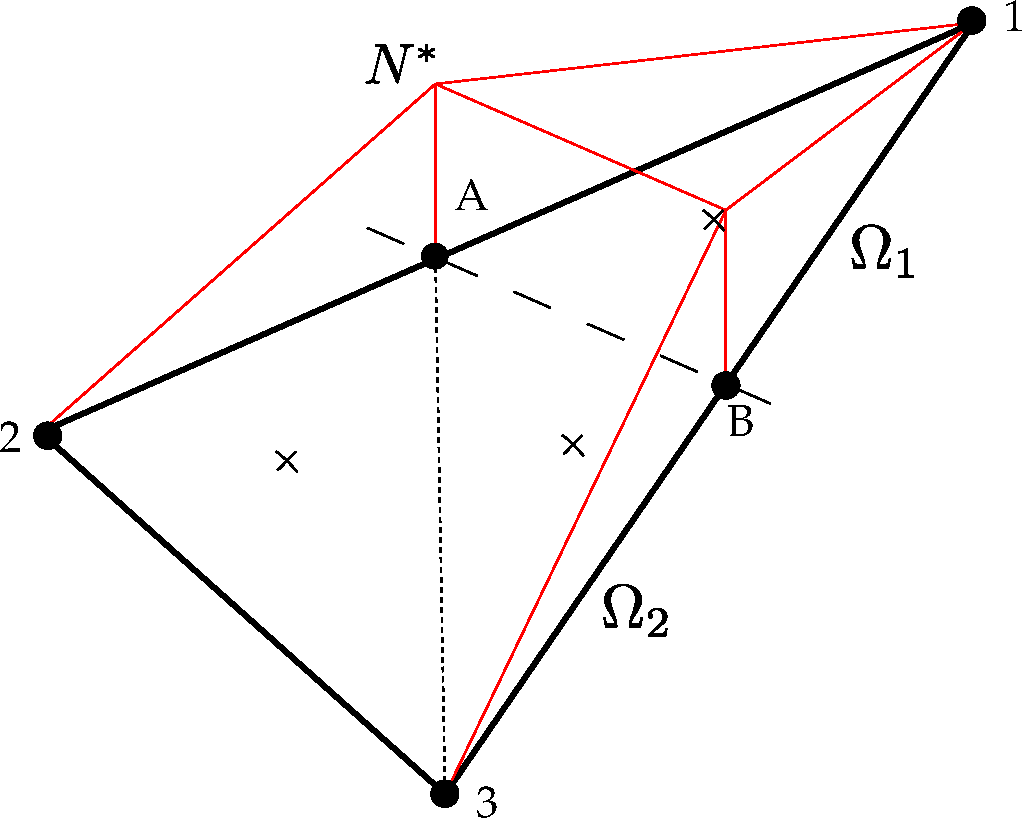
\includegraphics[width=.9\columnwidth]{images/enrichment1.pdf}
   \caption{2D interface element. The interface is calculated cutting the element with the segment $A-B$. The enrichment proposed by Coppola and the partition of the triangle into three sub-triangles with its own Gauss points to allowing to calculate an enhanced integration is shown.}
   \label{fg:enrichment1}                %% Etiqueta para la figura entera
\end{figure}

The second set of enrichment functions used in this work is described in Figure \ref{fg:enrichment2}. As in the previous case, the two new degrees of freedom can also be statically condensed. However, using this space it is possible to ensure continuity between elements, but paying the cost of having to rebuild the system matrix at each time step, which could be an expensive task due to memory allocation.
This enrichment space is constructed following
\begin{equation}
   \left\{\;
   \begin{matrix}
     \phi_A^*(\xx_A)=\phi_B^*(\xx_B)=1 \\
     \phi_A^*(\xx_1)=\phi_A^*(\xx_2)=\phi_A^*(\xx_3)=\phi_A^*(\xx_B)=0 \\
     \phi_B^*(\xx_1)=\phi_B^*(\xx_2)=\phi_B^*(\xx_3)=\phi_B^*(\xx_A)=0
   \end{matrix}\;
   \right.
   \label{eq:enrich-2a}
\end{equation}

\begin{figure}[H]
  \centering
   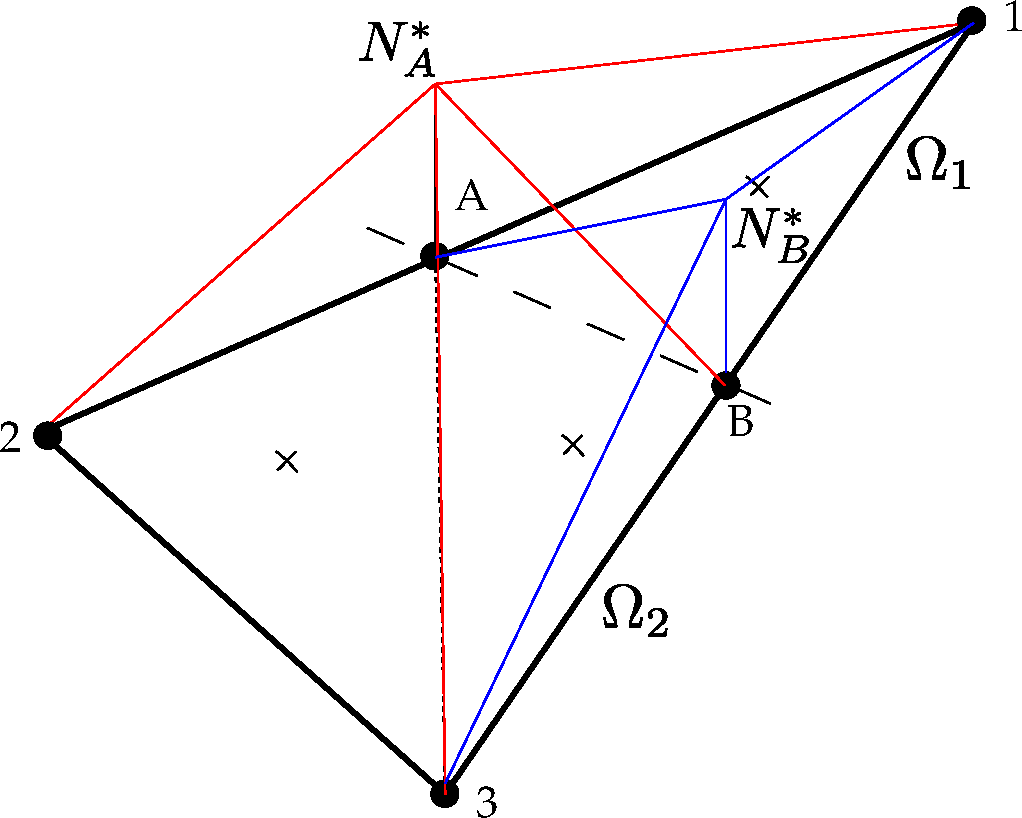
\includegraphics[width=.9\columnwidth]{images/enrichment2.pdf}
   \caption{2D interface element. The interface is calculated cutting the element with the segment $A-B$. An enrichment space with two functions per interface element, which can be used to ensure continuity between elements, is presented. The integration partition is the same as presented above (Figure \ref{fg:enrichment1}).}
   \label{fg:enrichment2}
\end{figure}

% \begin{figure}[H]
%   \centering
%     \subfloat[]{
% 	  \label{fg:enrichment1}         %% Etiqueta para la primera subfigura
% 	  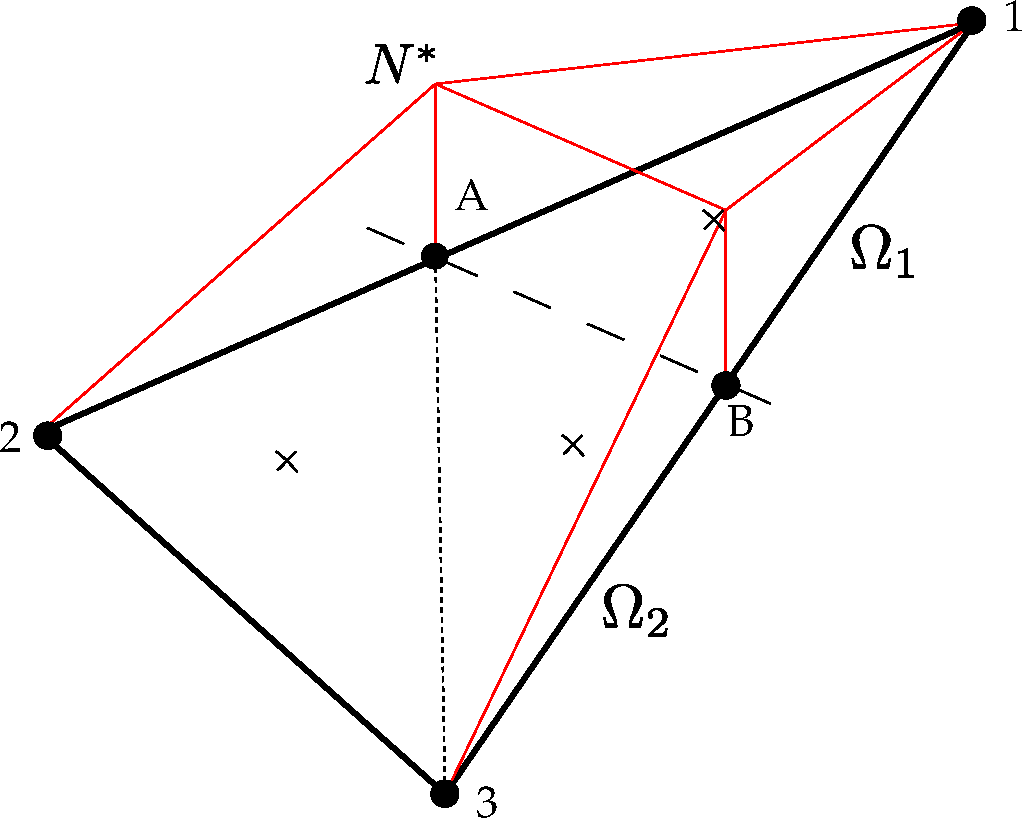
\includegraphics[width=.9\columnwidth]{images/enrichment1.pdf}
%     } \\
%     %%----segunda subfigura----
%     \subfloat[]{
% 	  \label{fg:enrichment2}         %% Etiqueta para la segunda subfigura
% 	  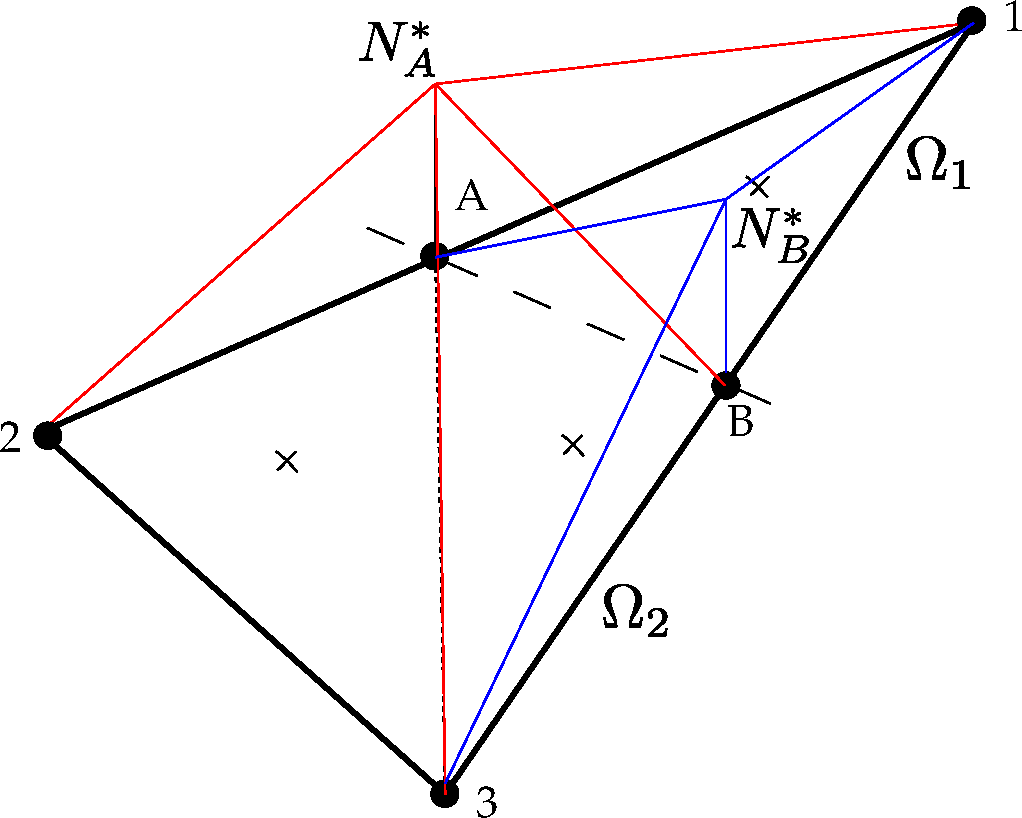
\includegraphics[width=.9\columnwidth]{images/enrichment2.pdf}
%     }
%    \caption{2D interface element. The interface is calculated cutting the element with the segment $A-B$. Figure \ref{fg:enrichment1} shows the enrichment proposed by Coppola and the partition of the triangle into three sub-triangles with its own Gauss points to allowing to calculate an enhanced integration. Figure \ref{fg:enrichment2} presents an enrichment space with two functions per interface element, which can be used to ensure continuity between elements. The integration partition is the same as presented above.}
%    \label{fg:enrichment}                %% Etiqueta para la figura entera
% \end{figure}

Therefore, using any of the enriched spaces, the pressure is now interpolated in the cut element following:
 \begin{equation}
      p_h(\xx) = \sum_{i=1}^{N_n} \phi_i(\xx) \ p_i + \sum_{i=1}^{N_e} \phi_i^*(\xx) \ p_i^*
   \end{equation}
where $\phi_i$ are traditional linear shape functions (a total of $N_n$), and $\phi_i^*$ are the enrichment shape functions (a total of $N_e$).

In order to capture the discontinuities and taking advantage of the enrichment functions used, the integration rules need to be modified in elements cut by the front. The method used is to divide each tetrahedral (triangular in 2D) element into up to six tetrahedral
(three triangular in 2D) sub elements. For each sub element the same integration rule as for the non-cut elements is used. Figure \ref{fg:enrichment1} shows that partition and the small circles represent the Gauss points for the integration. When using enrichment functions for the pressure, the material properties $\rho$,$\mu$ are taken as $\rho_1$,$\mu_1$ or $\rho_2$,$\mu_2$, depending on which part of the domain ($\Omega_1$ or $\Omega_2$) the integration point is found.

   \subsection{Pressure Calculation}

Particles can move across several elements and through the interface during a time-step, then the pressure gradient of the previous time-step would introduce a poor and even unstable approximation of the pressure forces. In order to avoid these large errors in the evaluation of the pressure gradients in the initial value of the iterative process, the value of the pressure is set to zero at the beginning of each time-step. Therefore, the acceleration over the particle calculated in X-IVAS stage is only is due to gravity force (pressure gradient is considered null and viscous forces are treated implicitly)\cite{Idelsohn13c}.

Starting from Equation \ref{Step5a}, and following the classical variational formulation, this is integrating, weighting with local shape functions and weakening both pressure laplacian and velocity divergence terms, it is possible to obtain the elemental contribution:

\begin{equation}
   \left[\Delta t \int_{\Omega^e} \frac{1}{\rho} \nabla \phi^T \nabla \phi \ d\Omega\right]\ \delta p^{n+1} = \left[\int_{\Omega^e} \nabla \phi^T \psi \ d\Omega\right]\ \hat \vv_j^{n+1}
\label{poisson}
\end{equation}
where the term resulting from weakening
\begin{equation}
\displaystyle \int_{\Gamma^e\cap\Gamma} \phi \left[ \hat \vv_j^{n+1} + \Delta t \frac{1}{\rho} \nabla  \delta p^{n+1} \right] \cdot \eta \ d\Gamma = \int_{\Gamma^e\cap\Gamma} \phi \ \vv_j^{n+1} \cdot \eta \ d\Gamma 
\end{equation}
 is zeroed to ensure impenetrability on walls.

The enrichment shape functions are used in the case of split elements, then the resulting system is:

  \begin{equation*}
   \begin{pmatrix}
      L_{\phi,\phi} & L_{\phi,*}\\
      {L_{\phi,*}}^T & L_{*,*}
   \end{pmatrix}\;
    \begin{pmatrix}
      \delta p^{n+1}\\
      \delta {p^*}^{n+1}
   \end{pmatrix}\; = \;
   \begin{pmatrix}
      D_{\phi}\\
      D_*
   \end{pmatrix}\;
   (\hat{\vv}^{n+1})
   \label{poisson}
\end{equation*}

where
\begin{itemize}
 \item ${(L_{\phi,\phi})}_{N_n\times N_n} = \Delta t \displaystyle \int_{\Omega^e} \dfrac{1}{\rho} \nabla \phi_i^T \nabla \phi_j \ d\Omega$
 \item ${(L_{\phi,*})}_{N_n\times N_e} = \Delta t \displaystyle \int_{\Omega^e} \dfrac{1}{\rho} \nabla \phi_i^T \nabla \phi_j^* \ d\Omega$
 \item ${(L_{*,*})}_{N_e\times N_e} = \Delta t \displaystyle \int_{\Omega^e} \dfrac{1}{\rho} \nabla {\phi_i^*}^T \nabla \phi_j^* \ d\Omega$
 \item ${(D_{\phi})}_{N_n\times N_n} = \displaystyle \int_{\Omega^e} \nabla \phi_i^T \psi_j \ d\Omega$
 \item ${(D_*)}_{N_n\times N_e} = \displaystyle \int_{\Omega^e}  \nabla {\phi_i^*}^T \psi_j \ d\Omega$
\end{itemize}

At this point is possible to choose between two options. First, if the enriched space \ref{eq:enrich-2a} is used, the new degrees of freedom can be included in the global system, which will guarantee continuity between elements. Second option is following the classical procedure of static condensation of the system through Gaussian elimination\cite{Felippa04}, where next reduced system is obtained:
  \begin{equation}
   \left[L_{\phi,\phi} - L_{\phi,*}{(L_{*,*})}^{-1}{L_{\phi,*}}^T\right](\delta p^{n+1}) = \left[D_{\phi}- L_{\phi,*}{(L_{*,*})}^{-1}D_{*}\right](\hat{\vv}^{n+1})
   \label{condensing}
  \end{equation}
with $\delta p^{n+1} = p^{n+1}-p^{n}$.

% --- INICIO PARRAFO IMPORTANTE A CORREGIR

Without ensuring continuity between elements, as it happens in the case of enriched ones when condensation is used, the assumption that the inter-elemental boundary terms from the weakening of the Poisson equation might be avoided is not true. From our experience, and like is reported by Coppola\cite{Coppola05}, when the Froude Number is high (this is, low density ratio), the forgotten term from the weakening of the divergence of the velocity introduces severe problems of numerical diffusion. A way to solve this problem is not integrating by parts the divergence term, but it requires imposing a pressure gradient on boundaries, whose value can not be easily predict when there is a gravitational field, large density ratio, and the fluid is not at rest. Finally, if condensation is used, we choose weakening the velocity divergence in the Poisson step only when large density ratio is considered. Continuous enrichment does not suffer of the above mentioned problems and the same formulation can be used for every 
Froude number. However, a loss of computational performance must be paid because the necessity of memory management to assemble the variable-size pressure equation system.

% --- FIN PARRAFO IMPORTANTE A CORREGIR

%   If we are interested in solving the system in absolute pressure terms, the final system is
% 
%   \begin{equation}
%   [L_{\phi,\phi} - L_{\phi,*}{L_{*,*}}^{-1}{L_{\phi,*}}^T](p^{n+1}) = [D_{\phi}- L_{\phi,*}{L_{*,*}}^{-1}D_*](\hat{\vv}^{n+1}) + [L_{\phi,\phi} - L_{\phi,*}{L_{*,*}}^{-1}{L_{\phi,*}^T] (p^n)
%    \label{condensing-abs}
%   \end{equation}

After obtain the new pressure, it is necessary to correct the velocity prediction using the pressure gradient. However, the new degree of freedom for the pressure must be taken into account in this step to calculate the enriched pressure gradient. In the case of condensed calculation, the value of $p*^{n+1}$ must be recovered from the nodal pressures calculated in the poisson step with:
\begin{equation}
  {p^*}^{n+1} = {(L_{*,*})}^{-1}[D_* \hat{\vv}^{n+1} - {L_{\phi,*}}^Tp^{n+1} + {L_{\phi,*}}^Tp^{n} + L_{*,*}{p^*}^n]
  \label{recovering}
\end{equation}

Finally, the equation system presented in Equation \ref{correction} must be solved.
 \begin{equation}
  \int_{\Omega} \psi \rho \vv^{n+1} d\Omega = \int_{\Omega} \psi \rho \hat{\vv}^{n+1} d\Omega - \Delta t \ \left[\int_{\Omega} \psi \nabla \delta p^{n+1} d\Omega + \int_{\Omega} \psi \nabla \delta {p^*}^{n+1} d\Omega \right]
  \label{correction}
 \end{equation}

Previously, it was mentioned that the pressure value is zeroed at the beginning of the time step. In the recovering step, one of the main reason can be found. It must be noticed that, not only the standard nodal pressures, but also the enrichments pressures of the previous iteration are required in this stage. Because the enrichment pressures depend on the location of the interface inside the element, using the latest $p^*$ of the previous time-step may introduce several problems due to the movement of the interface. This lead to poor results that in most cases become unstable.

Although this reinitialization of the pressure leads to a first iteration where the pressure calculation is of first order, further iterations pressure-correction improve the incompressibility of the solution. Idelsohn\cite{Idelsohn13c} ensures that this implies that the stabilization effect of the first order fractional step is lost due to the higher order scheme. We arrived to the same conclusion, because only two or three iterations are needed in order to obtain pressure convergence and, despite not being theoretically stable, pressure oscillations do not appear in the solution. Then, no stabilization technique is required in this case.
\subsection{PFEM-2 algorithm for two immiscible and incompressible fluids}

Considering details presented in above section for the treatment of free-surface, the main changes regarding to the general algorithm described in Section \ref{GeneralFor} are:
\begin{itemize}
  \item Implicit solution of viscosity terms: $\theta=1$
  \item Pressure restarting: $p^n=0$
\end{itemize}
As the initial pressure $p^n$ and the factor $1-\theta$ are both zero, the first stage of the general formulation can be suppressed and the algorithm starts with the X-IVAS step where the acceleration is only due to body forces $\mathbf{f}$. Finally, the Algorithm \ref{program:twofluids} presents the current PFEM algorithm to solve incompressible fluids with two different densities.

 \begin{program}[htbp]
	{\footnotesize
	\begin{enumerate}
	    \item X-IVAS Stage:
	    \begin{equation}
	      \left\{\;
	      \begin{matrix}[l]
		  \mathbf{x}^{n+1}_{p}=\mathbf{x}^{n}_{p}+ \sum_{i=1}^{N} \mathbf{v}^{n}(\mathbf{x}^{n+\frac{i}{N}}_{p}) \delta t \\
		  \widehat{\widehat{\mathbf{v}}}^{n+1}_{p}=\mathbf{v}^{n}_{p}+ \sum_{i=1}^{N} \mathbf{f}^{n} (\mathbf{x}^{n+\frac{i}{N}}_{p})  \delta t \\
		  \lambda_p^{n+1} =\lambda_p^n
	      \end{matrix}\;
	      \right.
	      \label{Step2step2fluids}
	    \end{equation}
	    \item Projection Stage:
	    \begin{equation}\label{Step3b2fluids}
	    \left\{\;
	      \begin{matrix}[l]
	      \displaystyle \widehat{\widehat{\mathbf{v}}}^{n+1}_{j}=\frac{\sum_{p} \widehat{\widehat{\mathbf{v}}}^{n+1}_{p} W(\mathbf{x}_{j}-\mathbf{x}_{p})}{\sum_{p} W(\mathbf{x}_{j}-\mathbf{x}_{p})} \\
	      \displaystyle \lambda^{n+1}_{j}=\frac{\sum_{p} \lambda^{n+1}_{p} W(\mathbf{x}_{j}-\mathbf{x}_{p})}{\sum_{p} W(\mathbf{x}_{j}-\mathbf{x}_{p})}
	      \end{matrix}\;
	      \right.
	    \end{equation}
	    \item Implicit Viscosity Stage:
	     \begin{eqnarray}\label{Step4a2fluids}
	      \displaystyle \int_{\Omega} \widehat{\mathbf{v}}^{n+1}_{j}\psi_j\ d\Omega =\int_{\Omega} \widehat{\widehat{\mathbf{v}}}^{n+1}_{j}\psi_j\ d\Omega + \theta \Delta t \int_{\Omega} \mu(\xx) \nabla^{2}\widehat{\mathbf{v}}^{n+1}_{j} \psi_j\ d\Omega
	      \end{eqnarray}

	    \item Pressure-Correction Iterations: \\
	    \texttt{set} $\mathbf{v}_j^n = \widehat{\mathbf{v}}^{n+1}_{j}$ \\
	    \texttt{for k=1 to K}
	    \begin{enumerate}
	     \item Poisson Stage: 
	     \begin{eqnarray}\label{Step5a2fluids}
	      \int_{\Omega} \nabla \cdot \left[\frac{\Delta t}{\rho(\xx)}\nabla(\delta p^{(n+\frac{k}{K})})\right]\phi_j\ d\Omega &=& \int_{\Omega} \nabla \cdot \mathbf{v}_j^{(n+\frac{k-1}{K})}\phi_j\ d\Omega
% 	      \\
% 	      \frac{\partial \delta p^{n+1}}{\partial n} &=& 0 \quad in \quad \Gamma_D \\
% 	      \delta p^{n+1} &=& 0 \quad in \quad \Gamma_N
	    \end{eqnarray}	    
	    \item Correction Stage:
	     \begin{multline}\label{Step5b2fluids}
	      \int_{\Omega} \psi \rho(\xx) \vv_j^{(n+\frac{k}{K})}\ d\Omega = \int_{\Omega} \psi \rho(\xx) \vv_j^{(n+\frac{k-1}{K})} d\Omega\\ 
	      - \Delta t \ \left[\int_{\Omega} \psi \nabla (\delta p)_j^{(n+\frac{k}{K})} d\Omega + \int_{\Omega} \psi \nabla {(\delta p^*)}^{(n+\frac{k}{K})}\ d\Omega\right]
	    \end{multline}
	    \end{enumerate}
	  \texttt{end for}
	  \item Particle Correction Stage:
	  \begin{equation}\label{Step6b}
	  \rho_p \mathbf{v}_p^{n+1}\  = \ \rho_p \widehat{\widehat{\mathbf{v}}}_p^{n+1} + \sum_{j} \delta \mathbf{v}_j^{n+1} \psi_j(\mathbf{x}_{p}^{n+1})
	  \end{equation}
	\end{enumerate}
	\caption{- Time-Step PFEM-2 for two immiscible and incompressible fluids.}
	\label{program:twofluids}
      }
      \end{program}


% \section{Second order improvements.}\label{Second_order}
% The well known \textit{Brezzi-BabÃŒska} condition (also called \textit{inf-sup} condition) determinates the interpolation families for the velocity and pressure to ensure stability and convergence in the Stokes problem. Originally, the PFEM-2 method uses the family P1/P1 (linear triangular elements) to approximate the variables $\mathbf{u}$ and $p$ on the mesh\cite{Idelsohn12b}. % because is a computationally cheap approach.
However, this family does not satisfy the \textit{inf-sup} condition, then it is unstable, so it requires to use stabilization at the Poisson step. Maybe carrying on the extra cost of the stabilization is possible, but using linear elements does not provided good accuracy with coarser meshes. Using finer meshes in PFEM-2 introduce another extra cost due to the necessity for use more particles to approximate the fields and update nodal values.

An alternative proposal is presented in this report. The idea is using the called Taylor-Hood finite elements\cite{HoodTaylor73}, which are presented in Figure \ref{fg:taylor-hood}. They consist on a quadratic approximation for the velocity and continuous linear approximation for pressure (family P2/P1). It is demonstrated that this family is stable because it satisfies the \textit{inf-sup} condition. However, that advantage could not be useful if the cpu-time required to reach some accuracy is larger than using P1/P1 elements.

\begin{figure}[htbp]
  \begin{center}
      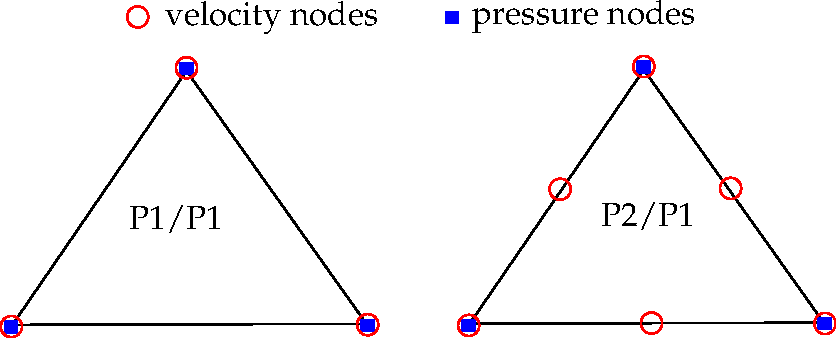
\includegraphics[width=.9\columnwidth]{images/taylor_hood.pdf}
  \end{center}
  \caption{\label{fg:taylor-hood} Left: Family P1/P1 originally used by PFEM-2. Right: Family P2/P1 proposed by this work.}
\end{figure}

\subsection{Square Cavity Tests}
% Previously, a new strategy to assemble the matrices and vectors of the linear equation systems was developed. It consists of pre-assembling the global matrices at the beginning of the simulation (for example mass and stiffness matrices), and after, at each time-step performing the final assemble with matrix-vector products. This approach improves the efficiency of the previous code (which assemble the matrices doing a loop over all the elements each time-step) in about a 20\%. However, it remains testing problems with variable coefficients.

% As we will see later, this approach is not useful for multi-fluids simulations, because the elemental matrices must be assembled each time-step and that formulation depends on the fluid zone that the element represents (interface zone or not).

Cartesian meshes were used for all cases. The name of the meshes indicates how many vertex-nodes there are in x-direction and y-direction respectly. For example the mesh \texttt{50x50-1ºorder} has 50 vertex-nodes in x-axis and 50 vertex-nodes in y-axis, conforming around 4800 first order triangular elements with 2500 degrees of freedom per variable. With second order grids have similar criteria, for example \texttt{25x25-2ºorder} has 25 vertex-nodes in each direction conforming 1250 second order triangular elements with approximately 2601 degrees of freedom per variable. Therefore the equation systems to solve with those meshes have approximately the same size.

\subsubsection{Re1000}

It was simulated using $\Delta t = 0.02$. Final simulation time $t_{final} = 50[s]$.

\begin{figure}[htbp]
  \begin{center}
      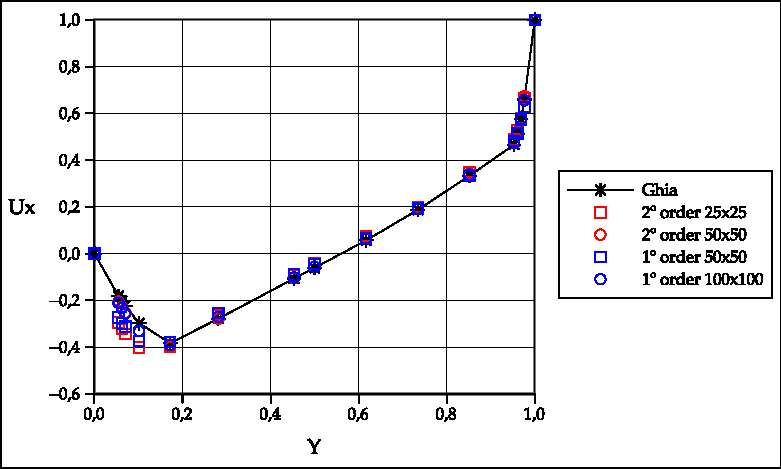
\includegraphics[width=.85\linewidth]{images/Re_1000_Ux.pdf}
      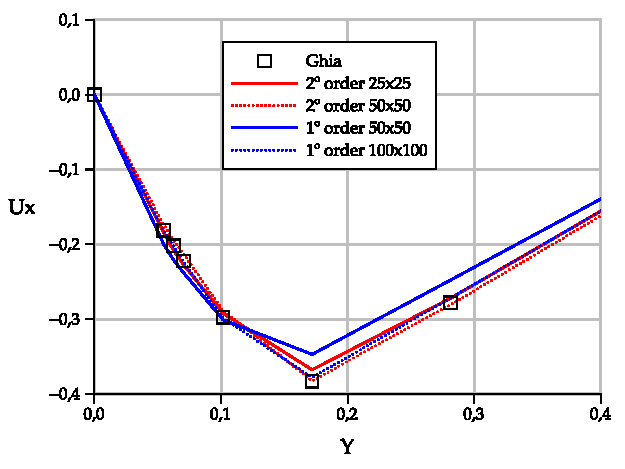
\includegraphics[width=.85\linewidth]{images/Re_1000_Ux_zoom.pdf}
  \end{center}
  \caption{\label{fg:Re1000u} Comparison with Ghia References at $Re=1000$. $u$ velocities at x-centerline.}
\end{figure}

\begin{figure}[htbp]
  \begin{center}
      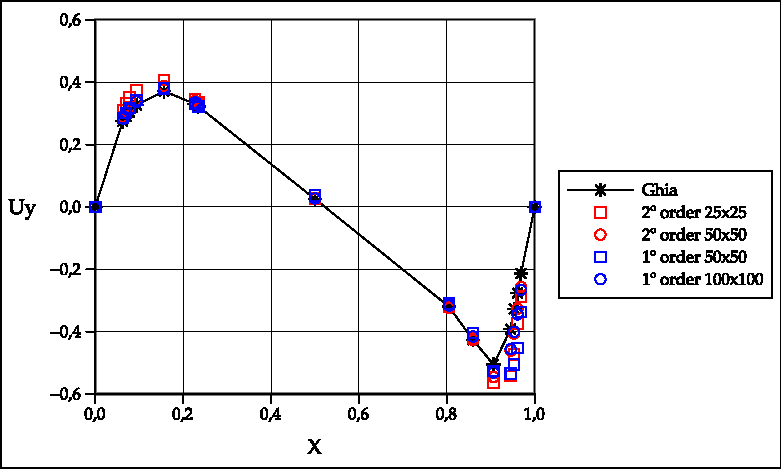
\includegraphics[width=.85\linewidth]{images/Re_1000_Uy.pdf}
      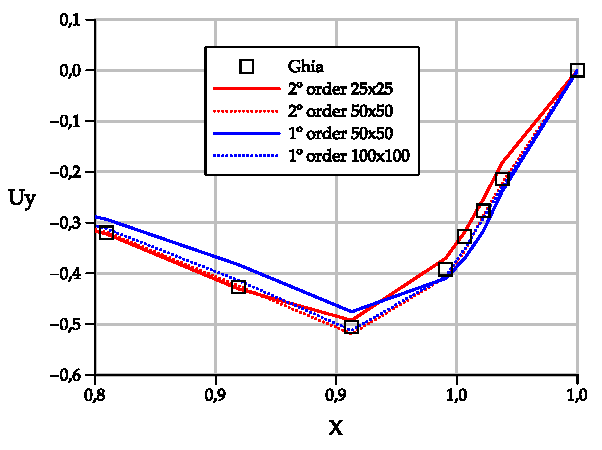
\includegraphics[width=.85\linewidth]{images/Re_1000_Uy_zoom.pdf}
  \end{center}
  \caption{\label{fg:Re1000v} Comparison with Ghia References at $Re=1000$. $v$ velocities at y-centerline.}
\end{figure}

\begin{table}[htbp]
\begin{center}
{\footnotesize
\begin{tabular}[h]{||c|c|c|c|c||}
    \hline
      Stage & $25x25$ - 2º order & $50x50$  - 2º order & $50x50$ - 1º order & $100x100$ - 1º order\\
      \hline
      \hline
	Acceleration & 34.6[s]& 134.58[s]& 22.8[s] & 97.9\\
	X-IVAS & 102.3[s]& 423.7[s]& 108.93[s] & 488.9 \\
	Projection & 32.4[s]& 153.8[s]& 75.0[s] & 359.1\\
	Poisson & 48.3[s]& 190.4[s]& 66.4[s] & 278.7\\
	Correction & 39.9[s]& 190.0[s]& 39.7[s] & 233.6\\
      \hline
	TOTAL & 257.57[s]& 1092.6[s]& 312.9[s] & 1458.1\\
      \hline
      \hline
	RMS $u$ & $2.0\times10^{-3}$ & $1.4\times10^{-3}$ & $5.8\times10^{-3}$ & $1.7\times10^{-3}$ \\
	RMS $v$ & $3.0\times10^{-3}$ & $2.2\times10^{-3}$ & $6.7\times10^{-3}$ & $2.4\times10^{-3}$ \\
      \hline
      \hline
\end{tabular}
}
\caption{\label{Tabla:times_Re_1000} Comparison table for CPU-times for the different PFEM-2 stages and the root mean square of the approximation error of $u$ and $v$. Case: $Re=1000$.}
\end{center}
\end{table}

\newpage

\subsubsection{Re 3200}


It was simulated using $\Delta t = 0.01$. Final simulation time $t_{final} = 100[s]$.

\begin{figure}[htbp]
  \begin{center}
      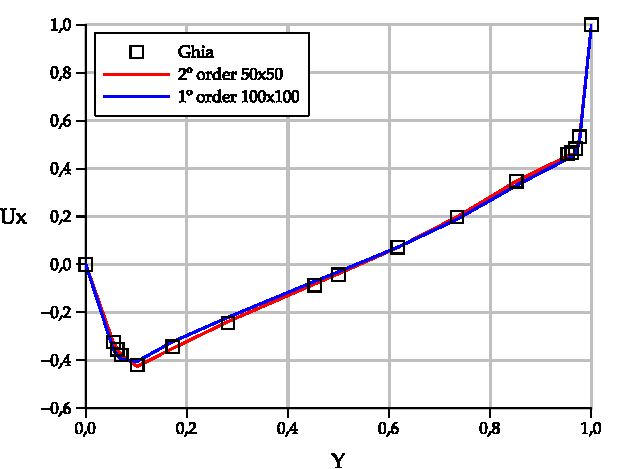
\includegraphics[width=.85\linewidth]{images/Re_3200_Ux.pdf}
      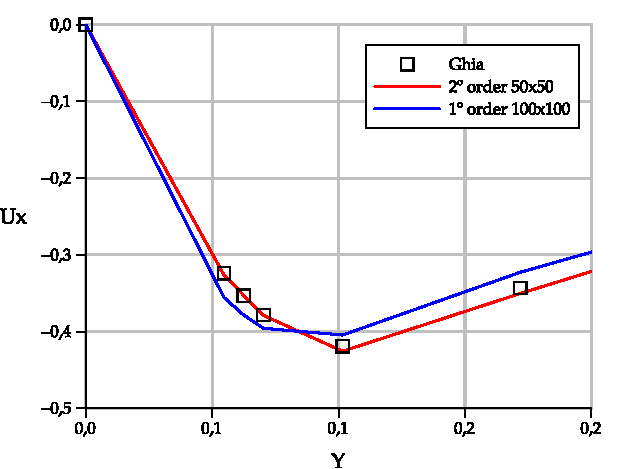
\includegraphics[width=.85\linewidth]{images/Re_3200_Ux_zoom.pdf}
  \end{center}
  \caption{\label{fg:Re3200} Comparison with Ghia References at $Re=3200$. $u$ velocities at x-centerline.}
\end{figure}

\begin{table}[htbp]
\begin{center}
{\footnotesize
\begin{tabular}[h]{||c|c|c||}
    \hline
      Stage & $50x50$  -2º order & $100x100$ - 1º order\\
      \hline
      \hline
	Acceleration & 134.9[s]& 98.01[s]\\
	X-IVAS & 427.5[s]& 499.9[s] \\
	Projection & 154.7[s]& 368.5\\
	Poisson & 191.1[s]& 283.6\\
	Correction & 189.2[s]& 242.9\\
      \hline
	TOTAL & 1097.4[s]& 1492.9\\
      \hline
      \hline
	RMS $u$ & 0.0106 & 0.0113 \\
      \hline
      \hline
\end{tabular}
}
\caption{\label{Tabla:times_Re_3200} Comparison table for CPU-times (to achieve $30[s]$ of real time) for the different PFEM-2 stages. Also the root mean square of the approximation error of $u$ at the end of the simulation is presented. Case: $Re=3200$.}
\end{center}
\end{table}

\newpage

\subsubsection{Re 10000}


It was simulated using $\Delta t = 0.01$. Final simulation time $t_{final} = 75[s]$.

\begin{figure}[htbp]
  \begin{center}
      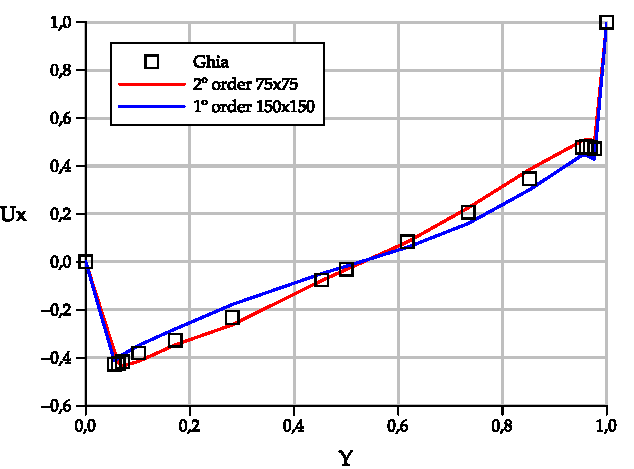
\includegraphics[width=.85\linewidth]{images/Re_10000_Ux.pdf}
  \end{center}
  \caption{\label{fg:Re10000} Comparison with Ghia References at $Re=10000$. $u$ velocities at x-centerline.}
\end{figure}


\begin{table}[htbp]
\begin{center}
{\footnotesize
\begin{tabular}[h]{||c|c|c||}
    \hline
      Stage & $75x75$  -2º order & $150x150$ - 1º order\\
      \hline
      \hline
	Acceleration & 515.0[s]& 367.1[s]\\
	X-IVAS & 1741.2[s]& 2114.1[s] \\
	Projection & 731.5[s]& 1651.2[s]\\
	Poisson & 740.9[s]& 1078.6[s]\\
	Correction & 911.4[s]& 1237.9[s]\\
      \hline
	TOTAL & 4640.0[s]& 6449.0[s]\\
      \hline
      \hline
	RMS $u$ & 0.015 & 0.0213 \\
      \hline
      \hline
\end{tabular}
}
\caption{\label{Tabla:times_Re_10000} Comparison table for CPU-times for the different PFEM-2 stages and the root mean square of the approximation error of $u$. Case: $Re=10000$.}
\end{center}
\end{table}

\newpage

\subsection{Summary}

  \begin{itemize}
   \item With the same number of nodes, second order achieve better accuracy than first order.
   \item With the same number of nodes, second order might be more efficient (it requires less elements and, then, less particles).
   \item The conclusion about the efficiency is only applicable to incompressible homogeneous flows with constant parameters (viscosity, density, etc). However, that asseveration can be modified when problems with non-constant diffusion-matrices will be required (turbulence modeling, multi-fluids. etc). Also several tests have demonstrated that the matrix storage is only useful for small or medium problems, but it is not applicable to large problems (more than 1M elements) because in those cases, it is slower than the traditional elemental assemble at each time step.
  \end{itemize}


\section{Results}\label{FS_results}

In this section, a wide range of free-surface problems with different ratio between densities and viscosities of the fluids involved are solved using the PFEM-2 method and the results compared with reference ones, which include numerical results, experimental analysis and/or analytical solutions.

The first case is the widely known Rayleigh-Taylor instability, where a small perturbation must generate complex fluid structures that are well reported in literature.
This problem focuses on the capabilities of the method to deal with large time-steps. These results are compared with those obtained with a well reputed Eulerian strategy, named Volume fo Fluid (VoF), which adds limiters as a method of guaranteeing boundedness of phase-fractions, and interface compression numerical terms to keep the interface sharp.
The second test is a sloshing problem which allows the numerical strategy behavior to be tested when different density ratios are simulated, the upcoming results are compared to well validated codes. In this second test, a discussion about the enrichment strategies is presented. Next, the ability of the method to deal with a highly dissipative free surface flow is tested with a standing wave problem, results are compared to semi-analytical solutions of the decayment of the total energy of the system.
Finally, the last example is a direct comparison against results coming from a dam-break experiment.
This case shows that the method can solve large motions of the interfaces and splashing of waves, while maintaining acceptable levels of accuracy when a comparison against pressure and height measurements is performed.

The main aim of this section is to show the capability of the method to work with large Courant numbers without stability loss and with negligible resign accuracy, reasonable large time-steps are then selected for each test. Previous PFEM-2 works (see \cite{Idelsohn12b}\cite{Gimenez14}), showed that the computational cost of each time-step is almost equal to traditional Eulerian solvers, and the increase of time-step decreases the duration of the global computation without loss of accuracy. Herein, the efficient distributed-memory implementation presented in \cite{Gimenez14} is extended to the free-surface treatment and used to simulate each of next cases presented.

 %if the method is able to solve simulation using larger time-steps than another codes, consequently it will be faster to solve the same problem and it will obtain results with guaranteed accuracy.

\subsection{Rayleigh-Taylor Instability}

This problem is based on the evolution of two layers of fluids initially at rest in a gravity field. The density of the upper most fluid is larger than the one placed underneath. Due to a little disturbance in the contact surface the more dense fluid moves down and the less dense fluid does the opposite. During the evolution of the problem, a mixture is created, which is lately segregated. The final state reaches an stable equilibrium with the more dense fluid at the bottom layer and the less dense fluid at the top layer. The growth and evolution of the instability has been investigated among others by Tryggvason\cite{Tryggvason88} for inviscid incompressible flows, and by Guermond \& Quartapelle\cite{Guermond00} for viscous flows.

The starting point is the problem documented by Guermond\cite{Guermond00}. The computational domain is $[-d/2,d/2]\times[-2d,2d]$ and the initial position of the perturbed interface is $\eta(x) = 0.1d \cos(2\pi x/d)$. The density ratio is $3$, which corresponds to an Atwood
number of $0.5$ according to Tryggvason's definition $At = (\rho_{max}-\rho_{min})/(\rho_{max}+\rho_{min})$. Other physical parameters are selected to obtain a Reynolds number $Re=\rho_{min}d^{\frac{3}{2}}g^{\frac{1}{2}}/\mu=1000$. The computational domain is discretized into $80000$ structured triangles ($\Delta x=0.01$) setting slip boundary conditions on each wall. The time step selected is $\Delta t=0.01[s]$, which allows for $CFL_{max} \approx 8$. Between five and eight particles per element are used and two pressure iterations are required.

To compare solutions with reference results, the time is made dimensionless by using $\widetilde{t} = t\sqrt{g\ At}$. Results on the vertical position of the tip of the falling and rising fluid (spike and bubble, respectively) are shown in Figure \ref{fg:rayleigh-rf}. It can be observed that current solution is in good agreement with the reference results.

\begin{figure}[H]
  \begin{center}
      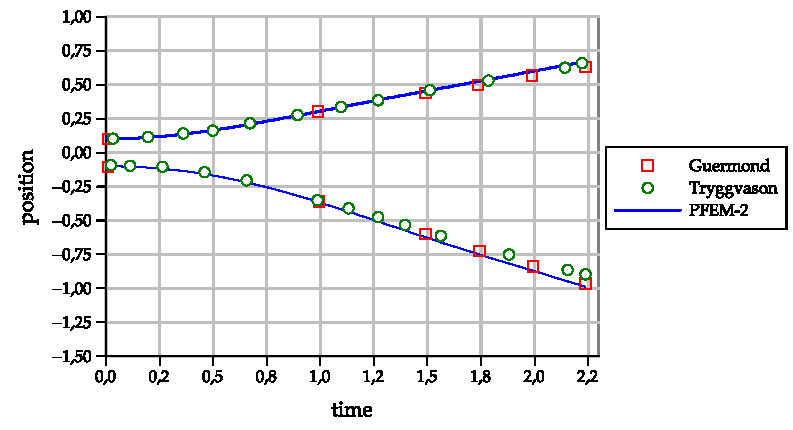
\includegraphics[width=\columnwidth]{images/rayleigh_1.pdf}
  \end{center}
  \caption{\label{fg:rayleigh-rf} Position of rising and falling bubbles versus time. Case with $Re=1000$.}
\end{figure}

On the other hand, the evolution of the instability is shown in Figure \ref{fg:rayleigh-screenshots} at dimensionless times $\widetilde{t}=0, 1, 1.5, 2$. Around $\widetilde{t}=1.5$ the heavy fluid begins to roll up into two counter-rotating vortices. Later, around $\widetilde{t} = 2$, these two vortices become unstable and a pair of secondary vortices appear at the tails of the roll-ups. These shapes of the fluid interface obtained with PFEM-2 are similar to the ones shown as reference results, see \cite{Guermond00}.


\begin{figure}[htbp]
  \begin{center}
      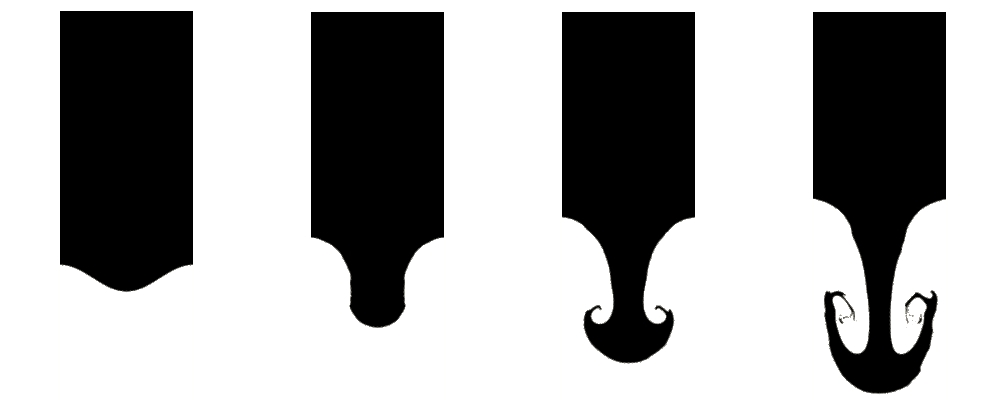
\includegraphics[width=\columnwidth]{images/rayleigh_2_better.jpg}
  \end{center}
  \caption{\label{fg:rayleigh-screenshots} Rayleigh-Taylor instability evolution. Case with $Re=1000$. From left to right $\widetilde{t} =0.0$, $1.0$, $1.5$, $2.0$.}
\end{figure}

\subsubsection{Extending the time step}

In order to emphasize the capability of the method to manage large time-steps, the current case is also simulated with a large range of $\Delta t$ using the in-house implementation of PFEM and comparing with results obtained by the widely known \OF suite. The problem setup and domain discretization is the same as presented above and the PFEM settings are not modified.

In the case of \OF, the solver \texttt{interFoam} is chosen, which implements a Volume of Fluid (VoF) algorithm for multiphase flow\cite{Berberovic09}\cite{Marquez2014}. It includes the multi-dimensional limiter for explicit solution (MULES) as a method of guaranteeing boundedness of scalar fields, in particular phase/mass-fractions (more information about MULES can be found in \cite{Marquez13}). Since \OF version 2.3, a new semi-implicit variant of MULES has been introduced which combines operator splitting with application of the MULES limiter to an explicit correction rather than to the complete flux. This approach would maintain boundedness and stability at an arbitrarily large Courant number. In the next simulation, the following recommended simulation schemes have been used: \texttt{CrankNicolson} (second order, implicit) time integration, \texttt{Gauss linear} (second order, Gaussian integration with linear interpolation) discretization for the gradient, divergence and Laplacian operators (\texttt{
corrected} with two \texttt{nNonOrthogonalCorrectors} due to the triangular mesh, for the later ). Relevant VoF settings are: \texttt{nAlphaSubCycles} is set in order to keep the CFL of the sub-cycling around $0.5$, \texttt{cAlpha}$=0.25$ to give more stability through relaxing on some level the strong sharpness imposition, and \texttt{MULESCorr} is enabled to calculate the limiter in a semi-implicit way.

Table \ref{fg:rayleigh-comparison-dts} presents the comparison of the solutions with PFEM and \OF at a particular time ($\widehat{t}=2.25$) using several fixed time-steps (with the largest time-step reaching a $CFL_{max}=15$). From captures, it can be shown that PFEM keeps approximately the same solution with each time-step, but interFoam can not solve with any accuracy using $\Delta t>0.001$ because the evolution of the mushroom-like interface differs form the reference results and this divergence is increased with larger time-steps. Moreover, simulations with interFoam diverge when $CFL_{mean}>0.5$ is reached (this happens at different times, depending on the selected time-step).


\begin{table}[H]
\begin{center}
\begin{tabular}{m{.18\textwidth} | >{\centering}m{.2\textwidth} | >{\centering}m{.2\textwidth} | >{\centering}m{.2\textwidth} | m{.2\textwidth} }
%       \hline
      Solver / $\Delta t$ [s] & 0.001 & 0.0025 & 0.01 & 0.025 \\
      \hline
      PFEM-2 &
      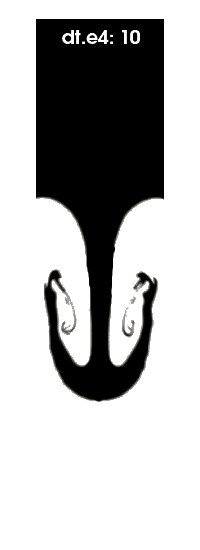
\includegraphics[width=.18\columnwidth]{images/rayleigh_pfem_dts_A.jpg} &
      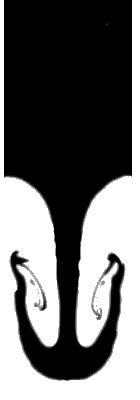
\includegraphics[width=.18\columnwidth]{images/rayleigh_pfem_dts_B.jpg} &
      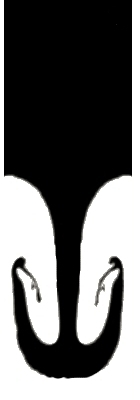
\includegraphics[width=.18\columnwidth]{images/rayleigh_pfem_dts_C.jpg} &
      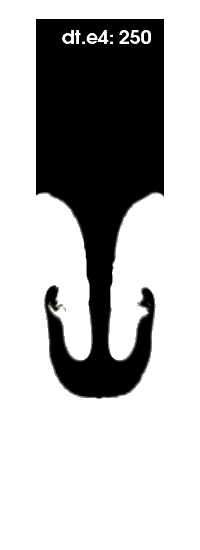
\includegraphics[width=.18\columnwidth]{images/rayleigh_pfem_dts_D.jpg}
      \\
%       \hline
      \OF &
      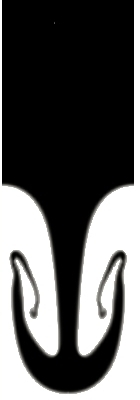
\includegraphics[width=.18\columnwidth]{images/rayleigh_foam_dts_A.jpg} &
      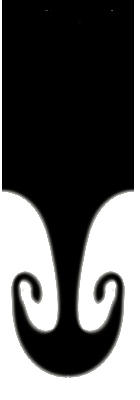
\includegraphics[width=.18\columnwidth]{images/rayleigh_foam_dts_B.jpg} &
      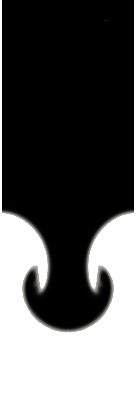
\includegraphics[width=.18\columnwidth]{images/rayleigh_foam_dts_C.jpg} &
      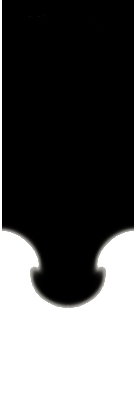
\includegraphics[width=.18\columnwidth]{images/rayleigh_foam_dts_D.jpg}
      \\
      \hline
\end{tabular}
\caption{\label{fg:rayleigh-comparison-dts} Rayleigh-Taylor instability captures for $\widetilde{t}=2.25$. \OF simulation implements VoF+MULES simulation  (\texttt{interFoam} solver).}
\end{center}
\end{table}
% 
% \begin{figure}[htbp]
%   \begin{center}
% 
%       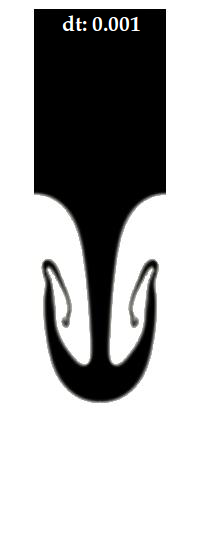
\includegraphics[width=.24\columnwidth]{images/rayleigh_foam_dts_A.png}
%       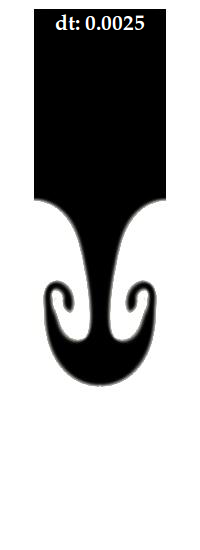
\includegraphics[width=.24\columnwidth]{images/rayleigh_foam_dts_B.png}
%       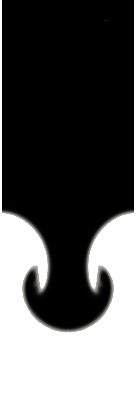
\includegraphics[width=.24\columnwidth]{images/rayleigh_foam_dts_C.jpg}
%       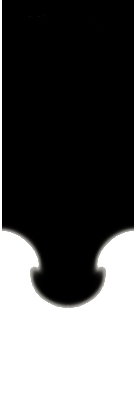
\includegraphics[width=.24\columnwidth]{images/rayleigh_foam_dts_D.jpg}
% 
%       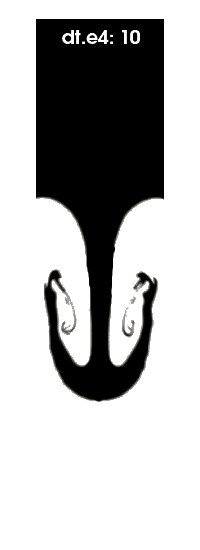
\includegraphics[width=.24\columnwidth]{images/rayleigh_pfem_dts_A.jpg}
%       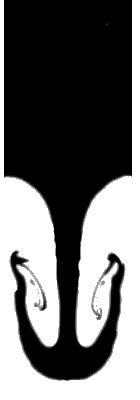
\includegraphics[width=.24\columnwidth]{images/rayleigh_pfem_dts_B.jpg}
%       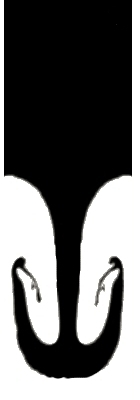
\includegraphics[width=.24\columnwidth]{images/rayleigh_pfem_dts_C.jpg}
%       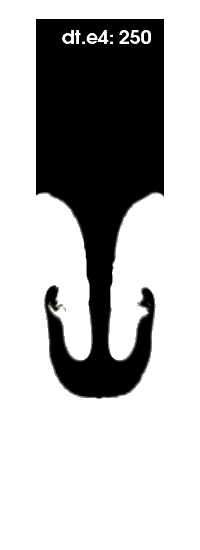
\includegraphics[width=.24\columnwidth]{images/rayleigh_pfem_dts_D.jpg}
% 
%   \end{center}
%   \caption{\label{fg:rayleigh-comparison-dts} Rayleigh-Taylor instability capture for $\widetilde{t}=2.25$. Bottom: PFEM simulations, top: VoF+MULES simulation (InterFoam solver - OpenFoam suite). From left to right $\Delta t =0.001[s]$, $0.0025[s]$, $0.01[s]$, $0.025[s]$.}
% \end{figure}

Another relevant feature to take into account when comparing both algorithms is that similar CPU times are required to solve a time-step.
Table \ref{tb:times-rt} summarizes the CPU Times required to complete $1[s]$ of real time in the current case. Results show that, using the same time-step, both solvers have similar performance, being \OF faster. However, due to the capability of time-step enlargement with PFEM, shorter CPU times are achieved with similar accuracy.

{\small
\begin{longtable}{||c|c||c||}
    \hline
    Solver & $\Delta t$ & CPU Time\\
      \hline
      \hline
      \OF & 0.001 & 1121[s]\\
      PFEM & 0.0025 & 1011[s]\\
      PFEM & 0.01 & 288[s]\\
      PFEM & 0.025 & 123[s]\\
      \hline
      \hline
    \caption{\label{tb:times-rt} Total computing times to simulate $1[s]$ of real time of the Rayleigh-Taylor instability 2d. Running on an Intel i5-3230M CPU @ 2.60GHz with 8Gb of RAM and one processor.}
\end{longtable}
}

\subsubsection{Three-dimensional simulation}

In this section, the extension of the two dimensional problem to three dimensions is presented. The third dimension is generated as a surface of revolution from the previous 2d geometry, conforming a cylindrical volume in 3d of radius $R=0.5$. This allows the same problem configuration to be kept, this is, a slip boundary condition on the wall, $At=0.5$, and an initial perturbation of the surface $\eta(r) = 0.1d \cos(2\pi r/d)$, with $0<r<R$.

The computational domain is discretized with a mesh size of $\Delta x=0.03[m]$ conforming a non-structured mesh with around $1.2$ millon tetrahedral elements. An average of eight millon particles are used during the simulation that move across the light-phase and heavy-phase domains. Simulation was carried out with a $\Delta t=0.025$ which peaks to $CFL_{max}=15$. Figure \ref{fg:rayleigh-3d} shows the evolution of the heavy-phase. It must be noticed that the simulation is extended until reaching the stable condition with the heavy-phase at the bottom and at rest, which is approximately $30[s]$ of simulation time. To complete the entire simulation, the implementation requires around three wall-clock hours running on an AMD Opteron 6376 @ 2.3GHz with a 64Gb RAM using 16 processors.

As an additional result, it is important to underline that, during the simulation, the global mass conservation has been verified.

 However, the spirit of this section is to show the stability of the 3D simulation with a realistic progress. A way to prove the validity of the solution is that, during the simulation, the initial mass quantity is preserved. A more detailed analysis about the accuracy of 3d simulations will be presented in Section \ref{sec:ETSIN-3d}.

\begin{figure}[htbp]
  \begin{center}
    \subfloat[]{
	  \label{fg:RT-3d-a}
	  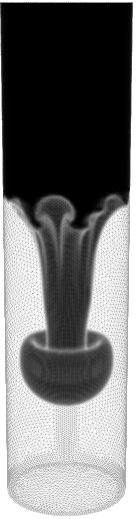
\includegraphics[width=.18\columnwidth]{images/RT_3d/RT3d_a.jpg}
    }
    \subfloat[]{
	  \label{fg:RT-3d-b}
	  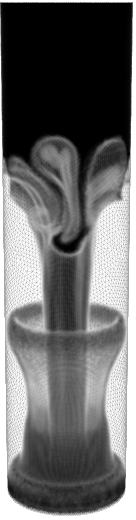
\includegraphics[width=.18\columnwidth]{images/RT_3d/RT3d_b.jpg}
    }
    \subfloat[]{
	  \label{fg:RT-3d-c}
	  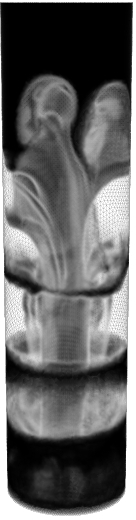
\includegraphics[width=.18\columnwidth]{images/RT_3d/RT3d_c.jpg}
    }
%     \subfloat[]{
% 	  \label{fg:RT-3d-d}
% 	  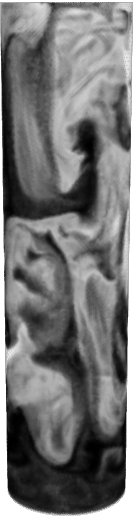
\includegraphics[width=.15\columnwidth]{images/RT_3d/RT3d_d.jpg}
%     }
    \subfloat[]{
	  \label{fg:RT-3d-e}
	  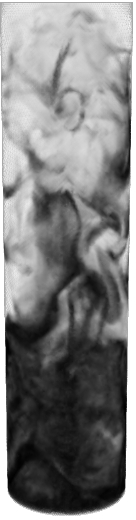
\includegraphics[width=.18\columnwidth]{images/RT_3d/RT3d_e.jpg}
    }
    \subfloat[]{
	  \label{fg:RT-3d-g}
	  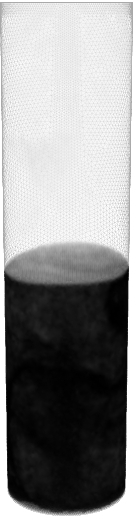
\includegraphics[width=.18\columnwidth]{images/RT_3d/RT3d_g.jpg}
    }
  \end{center}
  \caption{\label{fg:rayleigh-3d} Snapshots of the heavy-phase in the Rayleigh-Taylor instability solved in three-dimensions with PFEM-2. %From left to right $\widetilde{t} =2[s]$, $3.3[s]$, $4.4[s]$, $6.6[s]$, $8,8[s]$, and $27.5[s]$.}
  From left to right $\widetilde{t} =2[s]$, $3.3[s]$, $4.4[s]$, $8,8[s]$, and $27.5[s]$.}
\end{figure}

\afterpage{\clearpage}

\subsection{Non-linear sloshing in a rectangular container}\label{sec:Ansari}

Free surface oscillations of a liquid confined in a closed container (sloshing phenomenon) are an important issue when large amounts of liquid are industrially transported. The phenomenon involves two fluids that share a free surface boundary separating them, normally the density of the upper fluid is several orders of magnitude less than the bottom one. This phenomenon has proven of great interest due to the fact that violent impacts of the fluid can affect the structural integrity of the container.

For the studied cases in this section, the sloshing phenomenon is produced by a horizontal harmonic excitation $x = a_h \sin (\omega_h t)$, where $a_h$ is the excitation amplitude and $\omega_h$ is the excitation frequency of the rectangular tank where the two fluid phases are contained. The tank is divided in two parts, the bottom part where there is water with a density of $\rho_{I} = 1000 [kg/m^3]$ and the top part which contains a fluid with different densities $\rho_{II} = 1.3, 50, 200, 800 [kg/m^3]$, depending on the studied case. The dimensions of the tank are $a$(width) by $b$(height) and the initial free surface is at height $h$ from the bottom of the tank, see Figure \ref{fg:ansari-config}. The free surface starts the simulation as a horizontal line and is subsequently deformed by the tank excitation and the flow dynamics.

\begin{figure}[H]
  \begin{center}
      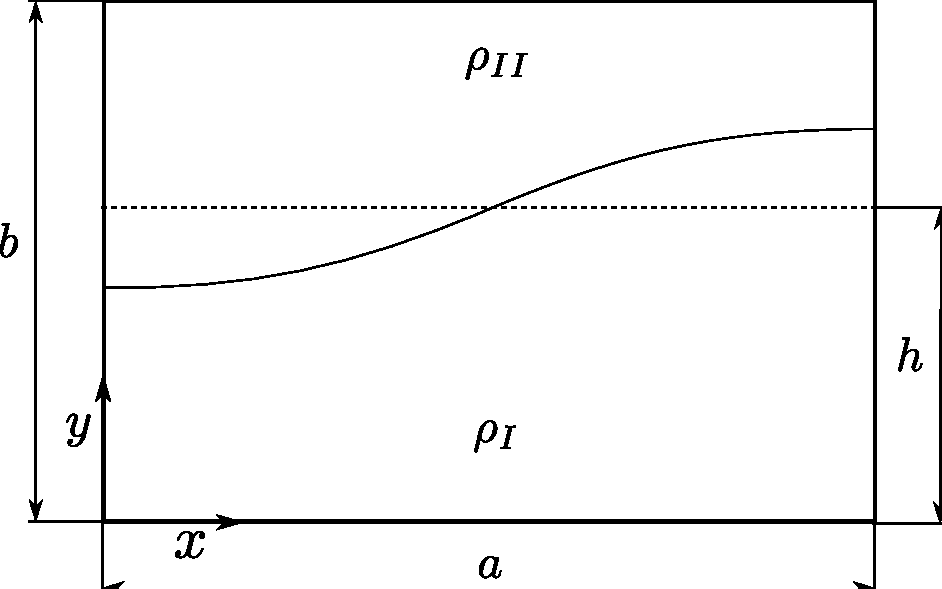
\includegraphics[width=.6\columnwidth]{images/ansari_config.pdf}
  \end{center}
  \caption{\label{fg:ansari-config} Configuration of the Non-linear sloshing in a rectangular container case. Initial condition is represented by a dashed line. The continuous line represents the position of the free-surface at a certain time.}
\end{figure}

For the different cases in this report, a 2D rectangular tank $a=1.0[m]$ width by $b=1.0[m]$ height is used. The initial height of the interface is $h=0.5[m]$ and the lateral excitation applied is $x=0.05\sin(3t)$. The simulations were performed considering the flow as laminar and non-viscous, hence, no turbulence model was included and slip boundary conditions are used. The inverse of the density ratio $\sigma=\frac{\rho{II}}{\rho{I}}$ was modified to study its influence on the free surface evolution. A two dimensional Cartesian mesh of $450\times225$, splitted into triangles, has been used in all cases.

Reference results for this case are taken from \cite{Goni13} which uses the codes STARCCM+ and \OF to obtain numerical solutions and reports the free surface displacement on the left wall of the container. Those simulations use the same grid as presented above, but, in order to avoid numerical instabilities, the $CFL$ number was limited to $CFL_{max}=0.5$ which implies $\Delta t \approx 0.001$. In PFEM-2 such restrictions do not exist, $\Delta t$ is therefore fixed to $0.01$, reaching a $CFL_{max}\approx5$.
Figure \ref{fg:ansari-results} presents the free surface displacement reported on the left wall of the container for different values of $\sigma$. For each one of them, PFEM-2 simulations show a good agreement with reference solutions. It is worth mentioning that the time step used is around ten times bigger than the one used in \cite{Goni13}.


  \begin{figure}[h]
  \centering
    \subfloat[]{
	  \label{fg:ansari-1}         %% Etiqueta para la primera subfigura
	  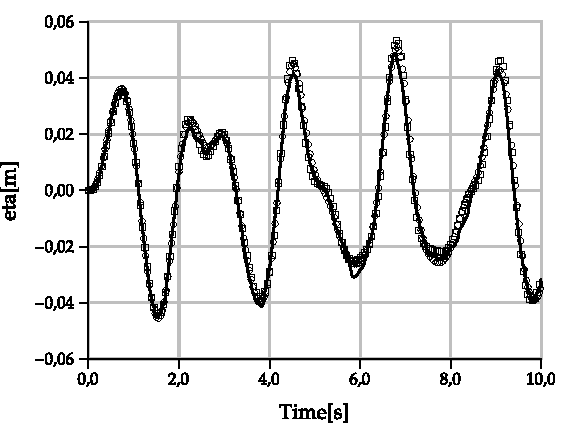
\includegraphics[width=.47\columnwidth]{images/ansari_1.pdf}
    }
    %%----segunda subfigura----
    \subfloat[]{
	  \label{fg:ansari-2}         %% Etiqueta para la segunda subfigura
	  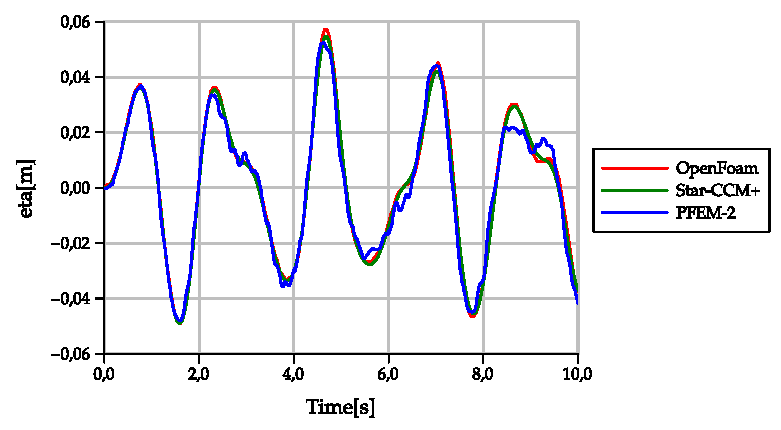
\includegraphics[width=.47\columnwidth]{images/ansari_2.pdf}
    } \\
    \subfloat[]{
	  \label{fg:ansari-3}         %% Etiqueta para la primera subfigura
	  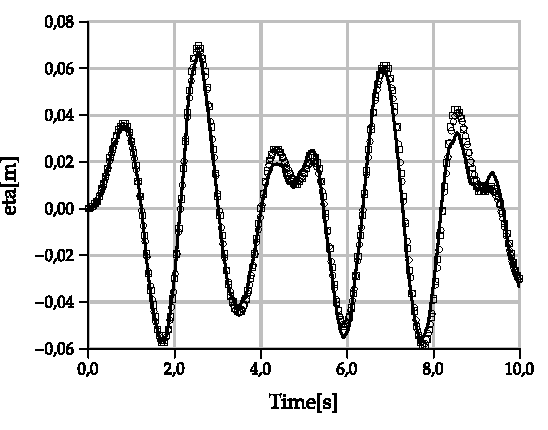
\includegraphics[width=.47\columnwidth]{images/ansari_3.pdf}
    }
    %%----segunda subfigura----
    \subfloat[]{
	  \label{fg:ansari-4}         %% Etiqueta para la segunda subfigura
	  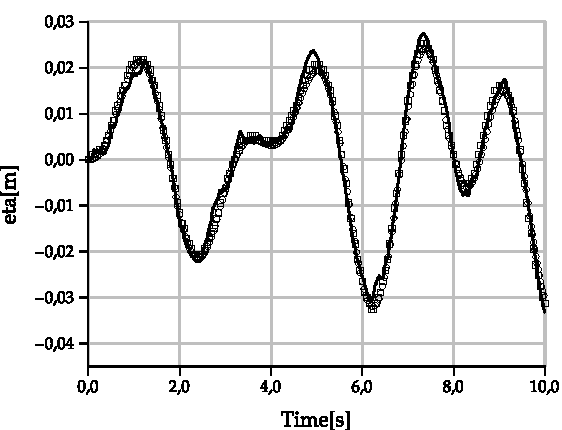
\includegraphics[width=.47\columnwidth]{images/ansari_4.pdf}
    }
   \caption{Level height on the left wall for a two phase flow for different density ratios. Figure \ref{fg:ansari-1}: $\sigma=0.0013$, Figure \ref{fg:ansari-2}: $\sigma=0.05$, Figure \ref{fg:ansari-3}: $\sigma=0.2$ and Figure \ref{fg:ansari-4}: $\sigma=0.8$. References:\ \Circle \ STARCCM, \Square \ OpenFOAM and filled line PFEM-2.}
   \label{fg:ansari-results}                %% Etiqueta para la figura entera
\end{figure}

\subsubsection{Enrichment and density ratio issues}

The PFEM-2 results presented in the previous section, have been obtained using the continuous enrichment strategy, which allows for the same formulation to be used, independently of the Froude number. However, as was mentioned before, without using a continuous formulation between elements for the enriched shape functions, the assumption about the inter-elemental boundary terms of the Poisson equation formulation should be revisited. In this subsection, problems that appear when the formulation combines non continuous enriched shape functions and low density ratio (approximately to one) are presented. The latter is somewhat measured by the Froude number, which also includes the ratio between inertial and gravitational forces, this is $Fr = \dfrac{U^2}{gL}\dfrac{\rho_I}{\rho_I-\rho_{II}}$. This phenomenon is mentioned, but not investigated, by Coppola\cite{Coppola05}.

Figure \ref{fg:ansari-results-b} shows a comparison between the level height calculated by PFEM-2 using continuous enrichment, discontinuous enrichment and no-enrichment for two extreme density ratio cases. It must be noted that next results were obtained with the enrichment shape functions presented in \ref{eq:enrich-1a}, however, using \ref{eq:enrich-2a}, and condensing the elemental matrices, similar conclusions were reached. The reference solution used in the Figure \ref{fg:ansari-results-b} was obtained using the formulation presented in \ref{eq:enrich-2a} without condensing, it is continuous enrichment. As it was mentioned, that reference solution was previously validated in section \ref{sec:Ansari}.

%Da la impresión que ambos sistemas de enrichment deberían ser discontinuos(??), pero el segundo es contínuo. -> Si bien el segundo sistema parece ser continuo, la continuidad va a depender de como lo ensamblas. Si haces condensación, aun utilizando el segundo enrichment te queda discontinuo. Si quieres continuidad hay que utilizar el segundo enrichment y NO condensar.

When both fluids have similar densities $\sigma \sim 1$, larger $Fr$ values are obtained. In Figure \ref{fg:ansari-4b} a comparison with $\sigma=0.8$ between different PFEM-2 formulations is presented. When no enrichment strategy is used, the solution
% \textcolor[rgb]{1.00,0.00,0.00}{
% at this high $Fr$ values
% }
presents a noisy behavior where, according to the level heights, a typical mass-loss appears, deteriorating the overall solution. When discontinuous enrichment is added (this is, condensing the equation system (\ref{eqsys-poisson})) the solution is smoother but still excessively dissipative compared to the continuous enrichment formulation used as reference. Meaning that, when the discontinuous enrichment formulation is used, the assumption of avoiding the inter-elemental boundary terms in the right hand side of (\ref{poisson}) is not correct and, consequently, a diffusive behavior appears. This conclusion is confirmed when discontinuous enrichment is used (but without weakening the divergence of the velocity) and a solution very similar to the continuous enrichment one is obtained (not presented in the figure for being almost identical to reference). By not integrating by parts, the divergence term requires imposing a pressure gradient on the boundaries: with low density ratios we can impose the previous gradient value $\nabla p^n$ on boundaries, although this approximation is not valid when there is a gravitational field, large density ratio, and the fluid is not at rest.

For the other limit $\sigma \ll 1$, the case when $\sigma=0.0013$, is presented in Figure \ref{fg:ansari-1b}. The graphic shows that both the continuous and the discontinuous enrichment solutions present very similar behavior. As before, when no enrichment is used, results become noisy, showing that a spurious velocity field appears close to the free surface when no improvements are introduced in this region. Discontinuous enrichment with strong form of divergence of the velocity is not possible to use in this case because the wrong prediction of pressure gradients on boundaries turns the simulation unstable.

  \begin{figure}[h]
  \centering
    \subfloat[]{
	  \label{fg:ansari-1b}         %% Etiqueta para la primera subfigura
	  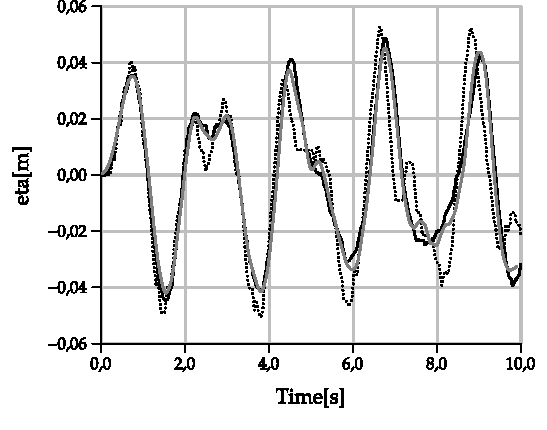
\includegraphics[width=.49\columnwidth]{images/ansari_1b.pdf}
    }
    %%----segunda subfigura----
    \subfloat[]{
	  \label{fg:ansari-4b}         %% Etiqueta para la segunda subfigura
	  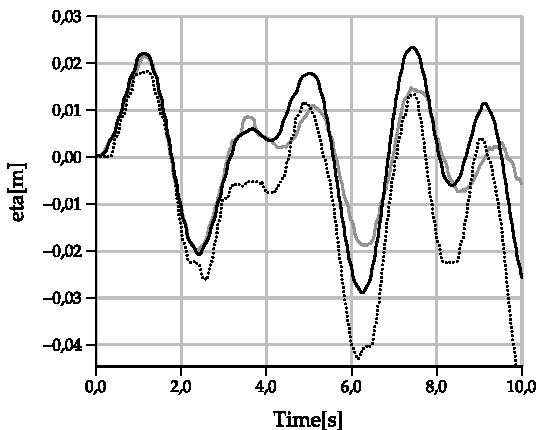
\includegraphics[width=.49\columnwidth]{images/ansari_4b.pdf}
    }
   \caption{Level height on the left wall of a two phase flow for different density ratios. Figure \ref{fg:ansari-1b}: $\sigma=0.0013$ and Figure \ref{fg:ansari-4b}: $\sigma=0.8$. References: filled black line continuous enrichment, filled gray line discontinuous enrichment, and dotted line without enrichment.}
   \label{fg:ansari-results-b}                %% Etiqueta para la figura entera
\end{figure}

In the current implementation, choosing the continuous enrichment formulation increases the total CPU time by $50\%$ compared to the other discontinuous formulations, albeit with the great advantage of being applicable to a wide range of situations. If the discontinuous enrichment formulation is used, better computing times are obtained. Nevertheless, some particularities, such as integrating the velocity divergence term by parts or not, must be taken into account depending on the density ratio of the problem.

\clearpage

\subsection{Viscous standing waves}%Re=250,2500.

Computing the dissipation due to wave-breaking remains a challenging problem in the computational fluid mechanics context. In order to analyze the PFEM-2 solution when two-phase viscous incompressible flows are simulated, the evolution of a viscous standing wave has been chosen. An approximate analytical solution is available for small amplitude perturbations in the scientific literature \cite{Lighthill01} and it is of practical interest since it is related to the propagation of gravity waves.

The chosen standing wave configuration consists in a rectangular tank with length $L$ and a water filling height of $H = L/2$. This setup has been extracted, see \cite{Colagrossi12}, Figure \ref{fg:standing-wave-config} for a sketch of this configuration. The wave length is $\lambda = L$, $k$ is the corresponding wave number (i.e. $k = 2\pi/\lambda$) and $A$ is the wave amplitude that defines the ratio $\epsilon=2A/H$.

\begin{figure}[H]
  \begin{center}
      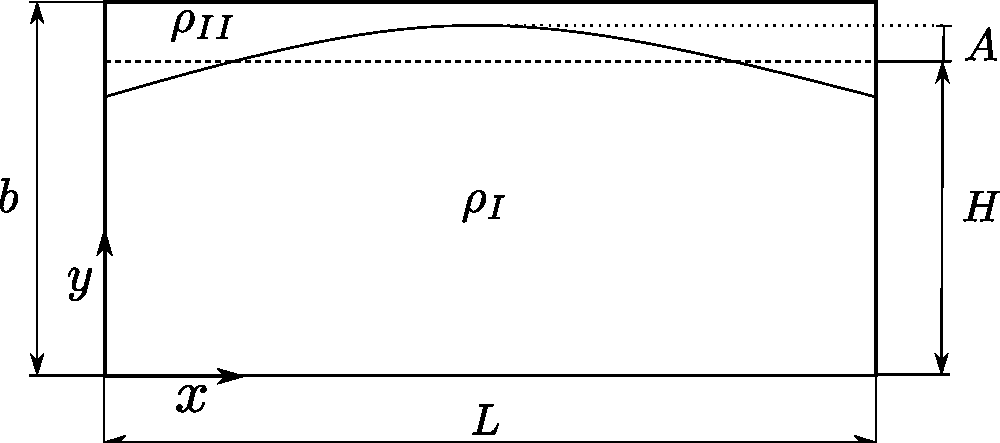
\includegraphics[width=.7\columnwidth]{images/standing_wave.pdf}
  \end{center}
  \caption{\label{fg:standing-wave-config} Configuration scheme of standing wave case. Initial condition is represented by dotted lines. In continuous line is presented an intermediate state where the maximum amplitude $A$ is reached.}
\end{figure}

When the fluid is viscous, solid boundary layers dissipation neglected, and assuming small-amplitude waves (i.e small $\epsilon$) and small wave steepness (i.e $2A/\lambda \ll 0.1$); an approximate analytical solution of the standing wave evolution can be obtained through the linearization of Navier-Stokes equations for traveling waves:
\begin{align}
 \varphi(x,y,t) & = \varphi_0(x,y)\cos(\omega t) \\
 \varphi_0(x,y) & =-\epsilon\frac{Hg}{2\omega}\frac{\cosh\left[k(y+H)\right]}{\cosh(kH)}\cos(kx)
\end{align}

where the circular frequency $\omega$ is given by the dispersion relation of gravity waves, that is, $\omega^2 = g k \tanh(kH)$ where $g$ is the acceleration of gravity. At time $t = 0$ the free surface is horizontal while the initial fluid velocity is given by $\varphi_0$.

It can be demonstrated that the approximate solution is well posed only for $Re\gg1$ and for $Re^{-1}\ll k \ll Re^{2/3}$, where $Re=H\sqrt{gH}/\nu$ is the Reynolds number for this problem. From that solution, it is possible to obtain the formula that gives the approximate decay of the kinetic energy\cite{Lighthill01}:

\begin{equation}
 \varepsilon_K(t) = \epsilon^2g\frac{\lambda H^2}{32}e^{-4\nu k^2t}\left[1+\cos(2\omega t)\right]
 \label{kin-eq}
\end{equation}

The kinetic attenuation is governed by the parameter $\beta_l = 4\nu k^2$, which depends on the wave number and on the kinematic viscosity $\nu = \mu/\rho_{I}$. Lately work\cite{Antuono13} has demonstrated that generally, the Equation (\ref{kin-eq}) overestimates the dissipations, especially when the Reynolds number is not very large. Then an improved damping rate is proposed in \cite{Antuono13} $\beta = 4\nu k^2 -  2\sqrt{2}k^{11/4}Re^{-3/2}+O(Re^{-2})$, which is next used for comparisons.

To accomplish the linear solution hypothesis, the PFEM-2 simulations have been implemented by using a free-slip condition for the velocity and a Neumann condition for the pressure along each boundary of the tank. Also, the parameters $L=2$, $A=0.05$ and $g=1$ have been selected.

Several Reynolds number ($Re=25,50,250,2500$) have been chosen to compare with the approximate analytic dissipation. Problems were solved using a grid size $\Delta x$ such that $H/\Delta x=100$ and varying $\Delta t$ in order to solve using a Fourier number $Fo=\frac{\nu\Delta t}{\Delta x^2}$ with a local maximum of $Fo_{max}\approx10-50$. Figure \ref{fg:sw-energy} shows the comparison between the expected energy dissipation (which includes the improved damping rate) and numerical results for kinetic energy calculated with PFEM-2. Large Fourier numbers were used in order to reduce the computation times required to complete the simulations showing that the accuracy of the method remains with large CFL numbers, even when large diffusion is considered.

  \begin{figure}[h]
  \centering
    \subfloat[]{
	  \label{fg:sw-energy-25}
	  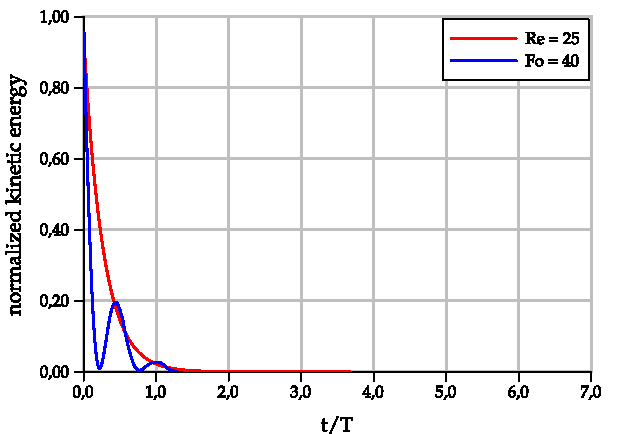
\includegraphics[width=.49\columnwidth]{images/sw_25.pdf}
    }
    \subfloat[]{
	  \label{fg:sw-energy-50}
	  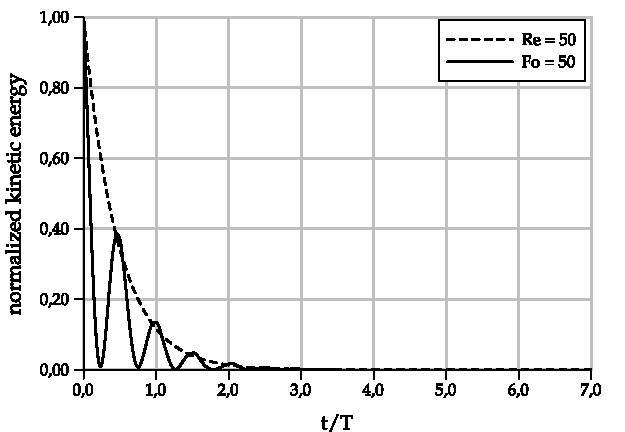
\includegraphics[width=.49\columnwidth]{images/sw_50.pdf}
    } \\
    \subfloat[]{
	  \label{fg:sw-energy-250}
	  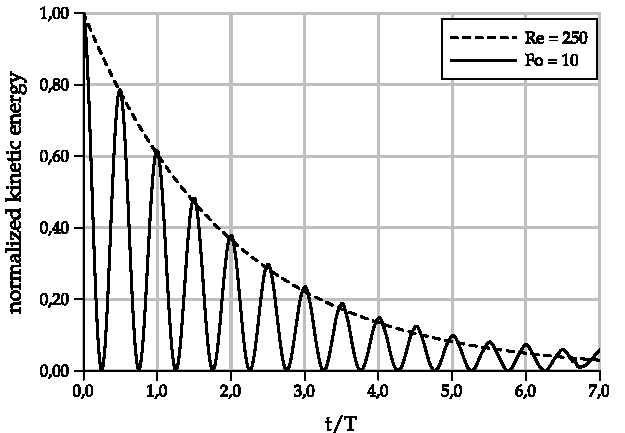
\includegraphics[width=.49\columnwidth]{images/sw_250.pdf}
    }
    \subfloat[]{
	  \label{fg:sw-energy-2500}
	  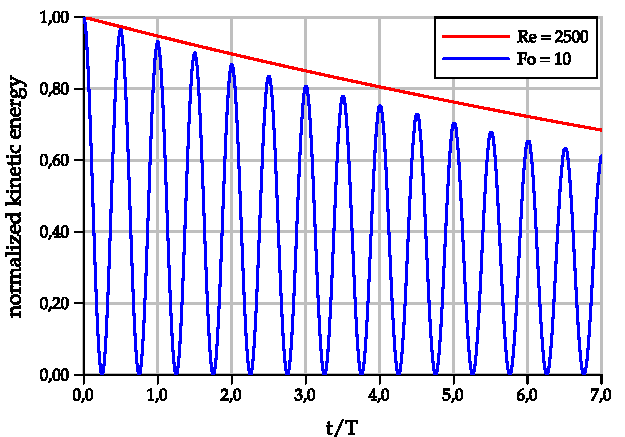
\includegraphics[width=.49\columnwidth]{images/sw_2500.pdf}
    }
   \caption{Kinetic Energy decay for standing wave problem with different Reynolds numbers. Dashed lines are approximate analytical solutions for total energy and filled lines are the kinetic energy calculated with PFEM-2. Reynolds numbers analyzed: $Re=25,50,250,2500$ in Figures \ref{fg:sw-energy-25},\ref{fg:sw-energy-50},\ref{fg:sw-energy-250},\ref{fg:sw-energy-2500} respectively. Legend in each figure indicates the maximum Fourier number used in each numerical simulation.}
   \label{fg:sw-energy}
\end{figure}
% \afterpage{\clearpage}

Regarding the computational effort, it is noticeable that the complete set of PFEM simulations have spent only few hours in an Intel i7-2600k 3.4GHz processor. This is a large difference with the CPU times reported in other works, see \cite{Colagrossi12}, where a similar set of problems were solved with similar accuracy using SPH and a 30 CPUs cluster, each CPU with 8 Intel Xeon 2.33GHz cores, running continuously for 30 days. 
\subsection{Dam-break problem}%ETSIN experimental tests

The objective of this section is to compare experimental measurements of a dam-break flow over a dry horizontal bed with the numerical approximation carried out with the PFEM-2 algorithm. The extensive set of experimental data is extracted from \cite{Lobovsky13}, where the dynamics of the dam break wave impacting a vertical wall downstream, with emphasis on the pressure loads and surface evolution after the dam burst, are presented.

A computational configuration of the tank used in experimental cases is presented in Figure \ref{fg:dambreak-config}, where the locations of water level measuring points and pressure sensors are shown. In this report, only the case with $H=300[mm]$ is analyzed. A two-phase non-viscous flow simulation is carried out, with $\rho_{water}=1000[kg/m^3]$, $\rho_{air}=1[kg/m^3]$ and gravity force $\mathbf{g}=-10\ \hat{j} [m/s^2]$. The 2D computational grid used has $322\times120$ nodes, conforming a mesh with around $80000$ triangles. Boundary conditions are slip on all walls, and $\Delta t$ is fixed to $0.1$, which allows for $CFL_{max}\approx20$ when the free surface impacts the downstream wall.

\begin{figure}[htbp]
  \begin{center}
      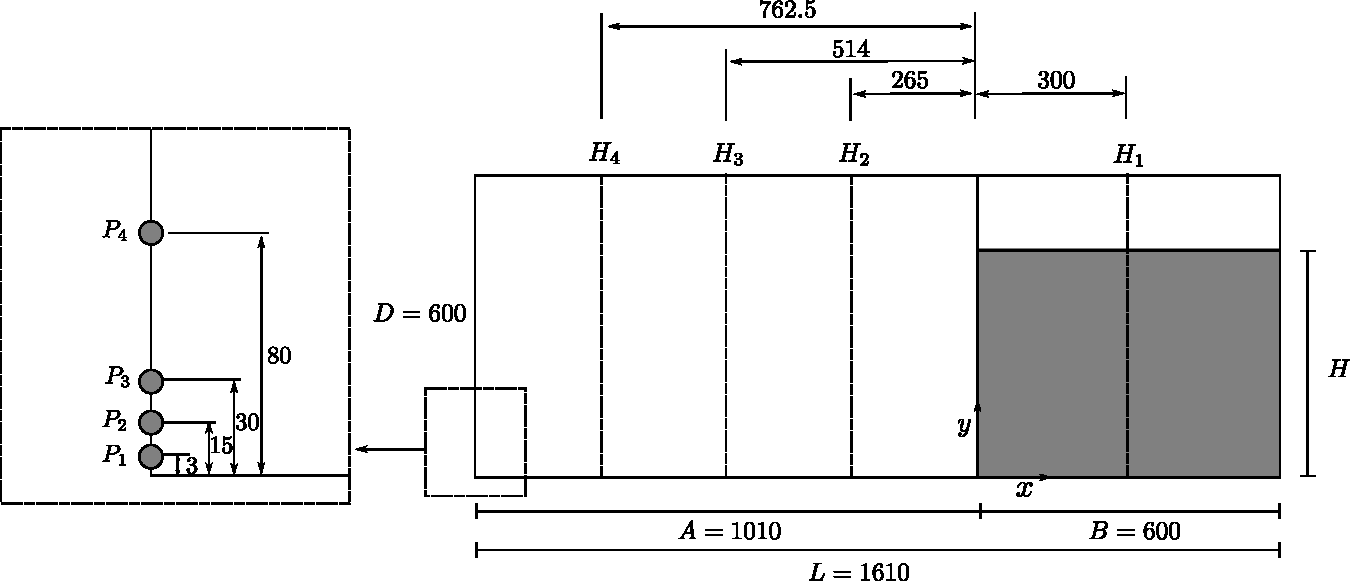
\includegraphics[width=\columnwidth]{images/dam_break_config.pdf}
  \end{center}
  \caption{\label{fg:dambreak-config} Configuration scheme of the dam-break case. $H_1$, $H_2$, $H_3$, $H_4$ present the locations of water level measuring positions. Also, $P_1$, $P_2$, $P_3$, $P_4$ show the locations of pressure sensors at the impact wall downstream from the dam. The grey zone represents the initial water condition. Dimensions are in millimeters.}
\end{figure}

Figure \ref{fg:dambreak-h} shows the comparison between experimental and numerical results for each water-level measurement. A good agreement can be observed, moreover when taking into account the capture of the back wave and splashing start events.
  \begin{figure}[h]
  \centering
    \subfloat[]{
	  \label{fg:dambreak-h1}         %% Etiqueta para la primera subfigura
	  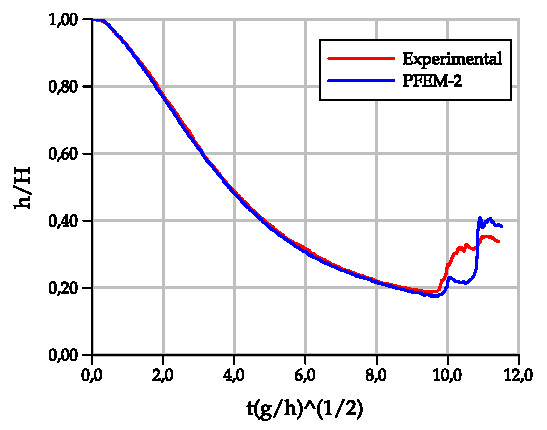
\includegraphics[width=.49\columnwidth]{images/dambreak_h1.pdf}
    }
    %%----segunda subfigura----
    \subfloat[]{
	  \label{fg:dambreak-h2}         %% Etiqueta para la segunda subfigura
	  \includegraphics[width=.49\columnwidth]{images/dambreak_h2.pdf}
    } \\
    \subfloat[]{
	  \label{fg:dambreak-h3}         %% Etiqueta para la primera subfigura
	  \includegraphics[width=.49\columnwidth]{images/dambreak_h3.pdf}
    }
    %%----segunda subfigura----
    \subfloat[]{
	  \label{fg:dambreak-h4}         %% Etiqueta para la segunda subfigura
	  \includegraphics[width=.49\columnwidth]{images/dambreak_h4.pdf}
    }
   \caption{Water levels at locations $H_1$, $H_2$, $H_3$ and $H_4$ for tests with initial filling height $H=300[mm]$ compared to data from literature experimental results\cite{Lobovsky13} (dashed lines) and numerical results with PFEM-2 (continuous lines). Time normalization is $t^*=t(g/h)^{1/2}$.}
   \label{fg:dambreak-h}                %% Etiqueta para la figura entera
\end{figure}

The impact pressure was measured with four sensors on the vertical wall at the end of the downstream flume, as described in Figure \ref{fg:dambreak-config}. The statistical analysis of the pressure peaks, rise times and the occurrence time, i.e. the time between
the opening of the dam gate and the occurrence of the impact, are presented in Figure \ref{fg:dambreak-p}. The shown pressure $P$ is non-dimensionalized with regards to the hydrostatic pressure at the bottom of the reservoir.

In the reference work, the analysis is focused on peak events. It can be noticed that the highest peak is recorded by sensor number 1 which is the sensor receiving the full impact, whilst the pressure of the other sensors is given by the run up of the flow. It can also be observed that sensor number 4, i.e. the sensor located at the highest position, does not show a pure impact event, see Figure \ref{fg:dambreak-p4}, and the maximum for this sensor is actually obtained later in time, when the water falls back after running along the wall. Numerical solution behavior follows the mentioned conclusions, although the pressure values are not between the statistical limits of experimental data. Also, a discrepancy can be observed with the peaks arrival times for sensors $1$ to $3$. This difference can be assigned to the numerical simplification which does not model the gate movement. However, the pressure magnitude of the peaks is well predicted giving confidence to PFEM-2 calculations.

  \begin{figure}[h]
  \centering
    \subfloat[]{
	  \label{fg:dambreak-p1}         %% Etiqueta para la primera subfigura
	  \includegraphics[width=.48\columnwidth]{images/dambreak_p4.pdf}
    }
    %%----segunda subfigura----
    \subfloat[]{
	  \label{fg:dambreak-p2}         %% Etiqueta para la segunda subfigura
	  \includegraphics[width=.48\columnwidth]{images/dambreak_p3.pdf}
    } \\
    \subfloat[]{
	  \label{fg:dambreak-p3}         %% Etiqueta para la primera subfigura
	  \includegraphics[width=.48\columnwidth]{images/dambreak_p2.pdf}
    }
    %%----segunda subfigura----
    \subfloat[]{
	  \label{fg:dambreak-p4}         %% Etiqueta para la segunda subfigura
	  \includegraphics[width=.48\columnwidth]{images/dambreak_p1.pdf}
    }
   \caption{Pressure time histories comparison between experimental results\cite{Lobovsky13} (discontinuous lines) and numerical results with PFEM-2 (continuous lines). Values at locations $P_1$, $P_2$, $P_3$, $P_4$ are presented in Figures \ref{fg:dambreak-p1},\ref{fg:dambreak-p2},\ref{fg:dambreak-p3},\ref{fg:dambreak-p4} respectively. Experimental results shows the median (dashed lines) and percentiles $2.5$ and $97.5$ (dotted lines).}
   \label{fg:dambreak-p}                %% Etiqueta para la figura entera
\end{figure}

Finally, Figure \ref{fg:dambreak-screenshots} presents snapshots for the evolution of the simulated free-surface. Initial condition is shown in Figure \ref{fg:dambreak-1}. Pressure peaks are related with the impact event observed in Figure \ref{fg:dambreak-3}, which generates the back wave propagation that is displayed in the remaining figures.
\begin{figure}[H]
  \centering
    \subfloat[]{
	  \label{fg:dambreak-1}
	  \includegraphics[width=.48\columnwidth]{images/dambreak_pfem_1_w.jpg}
    }
    %%----segunda subfigura----
    \subfloat[]{
	  \label{fg:dambreak-2}
	  \includegraphics[width=.48\columnwidth]{images/dambreak_pfem_2_w.jpg}
    } \\
    \subfloat[]{
	  \label{fg:dambreak-3}
	  \includegraphics[width=.48\columnwidth]{images/dambreak_pfem_3_w.jpg}
    }
    %%----segunda subfigura----
    \subfloat[]{
	  \label{fg:dambreak-4}
	  \includegraphics[width=.48\columnwidth]{images/dambreak_pfem_4_w.jpg}
    }\\
        \subfloat[]{
	  \label{fg:dambreak-5}
	  \includegraphics[width=.48\columnwidth]{images/dambreak_pfem_5_w.jpg}
    }
    %%----segunda subfigura----
    \subfloat[]{
	  \label{fg:dambreak-6}
	  \includegraphics[width=.48\columnwidth]{images/dambreak_pfem_6_w.jpg}
    } \\
    \subfloat[]{
	  \label{fg:dambreak-7}
	  \includegraphics[width=.48\columnwidth]{images/dambreak_pfem_7_w.jpg}
    }
    %%----segunda subfigura----
    \subfloat[]{
	  \label{fg:dambreak-8}
	  \includegraphics[width=.48\columnwidth]{images/dambreak_pfem_8_w.jpg}
    }
   \caption{Snapshots of the dam-break at times $t=0$, $0.25$, $0.5$, $0.75$, $1$, $1.25$, $1.5$, $1.75[s]$, in Figures \ref{fg:dambreak-1} to \ref{fg:dambreak-8} respectly.}
   \label{fg:dambreak-screenshots}
\end{figure}
\clearpage

\subsubsection{Three-dimensional Simulation}\label{sec:ETSIN-3d}

Despite being a problem that can accurately be simulated in 2D, the same example was run in 3D to test the ability of the PFEM-2 solver to deal with larger geometries and 3D problems. The 3D mesh, which adds a third dimension of a thickness of $0.15[m]$ with slip walls, has six million elements. These have an average $h=0.07$, demanding more than $25$ million particles for the fixed mesh approximation that fill the air and water domains. The same physical and numerical parameters of the 2D simulation were used. Sensors are placed in the same position on the left wall and in the middle position of the third dimension, see Figure \ref{fg:dambreak-config}.

In this example, the time step used, the element sizes and the velocity of the fluid lead to a simulation with some time-steps having a Courant number larger than 12, mainly when waves impact with walls. This shows once more, the capability of the method to manage 3D geometries with large time-steps. In Figure \ref{fg:dambreak-p-3d}, the pressure history for each sensor is presented, showing a similar appearance to the two dimensional simulation.

  \begin{figure}[h]
  \centering
    \subfloat[]{
	  \label{fg:dambreak-p1-3d}         %% Etiqueta para la primera subfigura
	  \includegraphics[width=.48\columnwidth]{images/dambreak_p4_3d.pdf}
    }
    %%----segunda subfigura----
    \subfloat[]{
	  \label{fg:dambreak-p2-3d}         %% Etiqueta para la segunda subfigura
	  \includegraphics[width=.48\columnwidth]{images/dambreak_p3_3d.pdf}
    } \\
    \subfloat[]{
	  \label{fg:dambreak-p3-3d}         %% Etiqueta para la primera subfigura
	  \includegraphics[width=.48\columnwidth]{images/dambreak_p2_3d.pdf}
    }
    %%----segunda subfigura----
    \subfloat[]{
	  \label{fg:dambreak-p4-3d}         %% Etiqueta para la segunda subfigura
	  \includegraphics[width=.48\columnwidth]{images/dambreak_p1_3d.pdf}
    }
   \caption{A pressure time history comparison between experimental results\cite{Lobovsky13} (discontinuous lines) and numerical results with PFEM-2 in three dimensions (continuous lines). Values at locations $P_1$, $P_2$, $P_3$, $P_4$ are presented in Figures \ref{fg:dambreak-p1-3d},\ref{fg:dambreak-p2-3d},\ref{fg:dambreak-p3-3d},\ref{fg:dambreak-p4-3d} respectively. Experimental results shows the median (dashed lines) and percentiles $2.5$ and $97.5$ (dotted lines).}
   \label{fg:dambreak-p-3d}                %% Etiqueta para la figura entera
\end{figure}
\clearpage


% \subsection{Sloshing roll}

As it was mentioned above, sloshing describes the movement of liquids inside partially filled tanks, generating dynamic loads on the tank structure. The resulting impact pressures are of great importance in assessing structural strength, and their correct evaluation still represents a challenge for the designer due to the high level of nonlinearities involved, with complex free surface deformations, violent
impact phenomena and influence of air trapping. In this section another two-dimensional case, is considered. Impact pressures at various critical locations induced by water motion in a partially filled rectangular tank, subject to a simple harmonic rolling motion, are evaluated and predictions are compared with experimental measurements\cite{Delorme07}\cite{Delorme09}.

Figure \ref{fg:roll-config} shows the selected 2d rectangular tank for the numerical simulations. In this work, one of the experiments of \cite{Delorme07} is analyzed, in which a sinusoidal rolling motion was imposed with an amplitude of $\theta=4º$ and a period $T=1.19[s]$. The rolling axis was located $18.4[cm]$ above the bottom line and the tank was fitted with a series of sensors, as indicated in Figure \ref{fg:roll-config}, but in this work the pressure corresponding to the most critical position is analyzed. Further details about the experiment are also found in \cite{Brizzolara11}.

\begin{figure}[H]
  \begin{center}
      \includegraphics[width=.75\columnwidth]{images/sloshing_roll.pdf}
  \end{center}
  \caption{\label{fg:roll-config} Configuration scheme of non-linear sloshing with harmonic rolling motion. Dimensions are in centimeters.}
\end{figure}

Computational grid used is composed with $180$ by $102$ nodes conforming a mesh with around $40000$ triangles. Boundary conditions are slip on each wall, and the initial condition is water at rest with $h=22.2[cm]$. The incompressible non-viscous multifluids PFEM solver with $\rho_{I}=1000[kg/m^3]$, $\rho_{II}=1000[kg/m^3]$ and $p_{\infty}=0[Pa]$ is used, choosing a time-step $\Delta t=0.01$.

Computational grid used is composed with $270$ by $153$ nodes conforming a mesh with around $84000$ triangles. Boundary conditions are slip on each wall, and the initial condition is water at rest with $h=22.2[cm]$. The incompressible non-viscous multifluids PFEM solver with $\rho_{I}=1000[kg/m^3]$ and $\rho_{II}=1000[kg/m^3]$ is used, choosing a time-step $\Delta t=0.01$.


\section{Conclusions}

The second generation of the Particle Finite Element Method (PFEM-2) is a contemporary strategy which uses a spatial discretization based on a background mesh and a cloud of particles. The dynamics equations are solved in a Lagrangian frame, where the implicit nonlinearities of the equation are solved using the {X-IVAS} strategy. That explicit temporal integration for convective terms allows for the use of large time-steps, thus providing a very efficient way when computing times are concerned.

% In the current work, a general formulation to solve free-surface flows with pressure gradient discontinuities was presented and exhaustively tested. That algorithm, which is based on a continuous enriched space for pressure, has shown good accuracy when solving a wide range of multiphase problems and keeping the advantage of the possibility to use large time-steps. Several cases with a large variety of Froude numbers, density ratios and dominant dissipative cases have also been analyzed. These results were compared with other reference softwares, semi-analytical expressions and also experimental data. In each of them, PFEM-2 has proven to be accurately competitive and computationally efficient. Regarding CPU times, they can be decreased without accuracy loss if the condensing strategy for enriched pressure degrees of freedom is used. Although that approach loses the generality of the formulation for any range of application, the computational cost enforcing the asseveration is reduced, which, to our knowledge, currently makes PFEM-2 the faster algorithm for solving multiphase flows.

In the current work, a formulation to solve free-surface flows with pressure gradient discontinuities, presented in \cite{Idelsohn13c}, was generalized and exhaustively tested. That algorithm, which is based on a continuous enriched space for pressure, has shown good accuracy when solving a wide range of multiphase problems and keeping the advantage of the possibility to use large time-steps. Several cases with a large variety of Froude numbers, density ratios and dominant dissipative cases have also been analyzed. These results were compared with other reference softwares, semi-analytical expressions and also experimental data. In each of them, PFEM-2 has proven to be accurately competitive and computationally efficient. Regarding CPU times, they can be decreased without accuracy loss if the original condensing strategy for enriched pressure degrees of freedom is used. Although that approach loses the generality of the formulation for any range of application, the computational cost enforcing the asseveration is reduced, which, to our knowledge, currently makes PFEM-2 the faster algorithm for solving multiphase flows.

% use section* for acknowledgement
\section*{Acknowledgment}

Authors thank to Pedro Gal\'an del Sastre (UPM-Spain), Eng. Pablo Becker (CIMNE-Spain), Dr. Norberto Nigro (CIMEC-Argentina) and Prof. Sergio Idelsohn (CIMNE-Spain and CIMEC-Argentina) for their valuable help and discussions about the method features and its implementation. Also to Dr. Santiago M\'arquez Dami\'an (CIMEC-Argentina) for his contribution in OpenFOAM simulations.

J. Gimenez gratefully acknowledges the support of the Argentinian Agencia Nacional de Promoci\'on Cient\'ifica y T\' ecnica (ANPCyT) through a doctoral grant in the FONCyT program. Also the authors would like to thank the program ERASMUS mundus action 2 ARCOIRIS project for their financial support throught a six-month doctoral scholarship.

Other financial support was provided by CONICET, Universidad Nacional del Litoral (CAI+D Tipo II 65-333 (2009)), ANPCyT-FONCyT (grants PICT 1645 BID (2008)) and ERC Advanced Grant REALTIME project AdG-2009325.

All the authors want to thank Mr. Hugo Gee for his valuable assistance during the preparation of this manuscript.

\bibliographystyle{plain}
\bibliography{mybib}


%\section{The Elsevier article class}
%
%\paragraph{Installation} If the document class \emph{elsarticle} is not available on your computer, you can download and install the system package \emph{texlive-publishers} (Linux) or install the \LaTeX\ package \emph{elsarticle} using the package manager of your \TeX\ installation, which is typically \TeX\ Live or Mik\TeX.
%
%\paragraph{Usage} Once the package is properly installed, you can use the document class \emph{elsarticle} to create a manuscript. Please make sure that your manuscript follows the guidelines in the Guide for Authors of the relevant journal. It is not necessary to typeset your manuscript in exactly the same way as an article, unless you are submitting to a camera-ready copy (CRC) journal.
%
%\paragraph{Functionality} The Elsevier article class is based on the standard article class and supports almost all of the functionality of that class. In addition, it features commands and options to format the
%\begin{itemize}
%\item document style
%\item baselineskip
%\item front matter
%\item keywords and MSC codes
%\item theorems, definitions and proofs
%\item lables of enumerations
%\item citation style and labeling.
%\end{itemize}
%
%\section{Front matter}
%
%The author names and affiliations could be formatted in two ways:
%\begin{enumerate}[(1)]
%\item Group the authors per affiliation.
%\item Use footnotes to indicate the affiliations.
%\end{enumerate}
%See the front matter of this document for examples. You are recommended to conform your choice to the journal you are submitting to.
%
%\section{Bibliography styles}
%
%There are various bibliography styles available. You can select the style of your choice in the preamble of this document. These styles are Elsevier styles based on standard styles like Harvard and Vancouver. Please use Bib\TeX\ to generate your bibliography and include DOIs whenever available.
%
%Here are two sample references: \cite{Feynman1963118,Dirac1953888}.
%
%\section*{References}
%
%\bibliography{mybibfile}

\end{document} 